\documentclass[12pt,a4paper,oneside]{report}

\usepackage[a4paper,margin=1in]{geometry}
\usepackage{setspace}
\usepackage{graphicx}
\usepackage{float}
\usepackage{booktabs}
\usepackage{longtable}
\usepackage{amsmath}
\usepackage{amssymb}
\usepackage{caption}
\usepackage{subcaption}
\usepackage{enumitem}
\usepackage{xcolor}
\definecolor{provablue}{RGB}{28, 69, 135}
\definecolor{provalight}{RGB}{235, 243, 250}

\usepackage[T1]{fontenc}
\usepackage{mathpazo} % Palatino font for a beautiful academic look
\usepackage{microtype} % Improves text justification
\usepackage{parskip} % Modern paragraph spacing instead of indentation

\usepackage{titlesec}
\usepackage{tikz}
\usetikzlibrary{shapes.geometric, arrows.meta, positioning}
\usepackage{listings}

\lstdefinelanguage{JavaScript}{
  keywords={typeof, new, true, false, catch, function, return, null, catch, switch, var, if, in, while, do, else, case, break, const, let, import, export, from, default, class},
  keywordstyle=\color{provablue}\bfseries,
  ndkeywords={class, export, boolean, throw, implements, import, this},
  ndkeywordstyle=\color{darkgray}\bfseries,
  identifierstyle=\color{black},
  sensitive=false,
  comment=[l]{//},
  morecomment=[s]{/*}{*/},
  commentstyle=\color{gray}\ttfamily,
  stringstyle=\color{purple}\ttfamily,
  morestring=[b]',
  morestring=[b]"
}

\lstdefinestyle{mystyle}{
    backgroundcolor=\color{provalight},
    commentstyle=\color{gray},
    keywordstyle=\color{provablue}\bfseries,
    numberstyle=\tiny\color{gray},
    stringstyle=\color{purple},
    basicstyle=\ttfamily\footnotesize,
    breakatwhitespace=false,
    breaklines=true,
    captionpos=b,
    keepspaces=true,
    numbers=left,
    numbersep=5pt,
    showspaces=false,
    showstringspaces=false,
    showtabs=false,
    tabsize=2,
    frame=single,
    rulecolor=\color{provablue}
}
\lstset{style=mystyle}
\titleformat{\chapter}[display]
  {\thispagestyle{empty}\vspace*{\fill}\normalfont\Huge\bfseries\centering\color{provablue}}
  {\chaptertitlename\ \thechapter}
  {20pt}
  {\Huge}
  [\vspace*{\fill}\clearpage]
\titlespacing*{\chapter}{0pt}{0pt}{0pt}

\newcommand{\frontmatterchapter}[1]{%
  \clearpage
  \titleformat{\chapter}[block]
    {\normalfont\Huge\bfseries\color{provablue}}
    {}
    {0pt}
    {}
  \titlespacing*{\chapter}{0pt}{0pt}{1em}
  \chapter*{#1}
  \addcontentsline{toc}{chapter}{#1}
  \titleformat{\chapter}[display]
    {\thispagestyle{empty}\vspace*{\fill}\normalfont\Huge\bfseries\centering\color{provablue}}
    {\chaptertitlename\ \thechapter}
    {20pt}
    {\Huge}
    [\vspace*{\fill}\clearpage]
  \titlespacing*{\chapter}{0pt}{0pt}{0pt}
}
\titleformat{\section}
  {\normalfont\Large\bfseries\color{provablue}}{\thesection}{1em}{}
\titleformat{\subsection}
  {\normalfont\large\bfseries\color{provablue}}{\thesubsection}{1em}{}

\usepackage{fancyhdr}
\setlength{\headheight}{25pt}
\pagestyle{fancy}
\fancyhf{}
\fancyhead[L]{\textcolor{provablue}{\slshape\leftmark}}
\fancyfoot[C]{\thepage}
\renewcommand{\headrulewidth}{0.4pt}
\renewcommand{\headrule}{\hbox to\headwidth{\color{provablue}\leaders\hrule height \headrulewidth\hfill}}

\usepackage[colorlinks=true, linkcolor=provablue, citecolor=provablue, urlcolor=provablue]{hyperref}
\usepackage[backend=biber,style=ieee]{biblatex}

\addbibresource{references.bib}

\newcommand{\projectname}{Prova}
\newcommand{\thesistitle}{\projectname: Virtual Try-On and AI Shopping Assistant for Fashion E-commerce}
\newcommand{\universityname}{Modern Academy}
\newcommand{\facultyname}{Faculty of Computer Science}
\newcommand{\departmentname}{Computer Science Department}
\newcommand{\degree}{Bachelor Graduation Project}
\newcommand{\submissiondate}{May 2026}
\newcommand{\universitylogosize}{3cm}

\begin{document}

\begin{titlepage}
    % PAGE 1: Project Team Page
    \begin{center}
        \includegraphics[width=\universitylogosize]{figures/university-logo.png}\par\vspace{0.5cm}
        {\Large\bfseries Modern Academy for Computer Science\\And Management Technology in Maadi\\Department: Computer Science.\par}
        
        \vspace{1.5cm}
        {\Large\bfseries B. Sc. Final Year Project\par}
        
        \vspace{1.5cm}
        {\Huge\bfseries \projectname\par}
    \end{center}
    
    \vspace{1.5cm}
    \begin{flushleft}
        {\Large\bfseries Team Members:\par}
        \vspace{0.3cm}
        \begin{itemize}[label=\textbullet, leftmargin=*]
            \item \large \textbf{Amro Rabea}
            \item \large \textbf{Yousef Ayman}
            \item \large \textbf{Seif Ezz Eldin}
            \item \large \textbf{Seif Eldin Mohamed}
            \item \large \textbf{Ahmed Mamdouh}
        \end{itemize}
        
        \vspace{1.5cm}
        \centering
        {\Large\bfseries Supervisors:\par}
        \vspace{0.3cm}
        {\large \textbf{Dr. Ahmed Ibrahim}\par}
        \vspace{0.2cm}
        {\large \textbf{Eng. Alaa Abouelela}\par}
    \end{flushleft}
    
    \vspace{1cm}
    \begin{center}
        {\Large\bfseries 2025-2026\par}
    \end{center}
    
    \clearpage

    % PAGE 2: Academy Vision & Mission
    \begin{flushleft}
        \includegraphics[width=\universitylogosize]{figures/university-logo.png}\par\vspace{0.5cm}
        {\Large\bfseries Modern Academy for Computer Science\\And Management Technology in Maadi\\Department: Computer Science.\par}
        
        \vspace{1.5cm}
        {\Large\bfseries Vision:\par}
        \vspace{0.5cm}
        {\large Modern Academy for Computer Science and Management Technology in Maadi vision is to achieve excellence in its fields of specialization to match the new local, regional, and international updates in the labor market.\par}
        
        \vspace{1.5cm}
        {\Large\bfseries Mission:\par}
        \vspace{0.5cm}
        {\large The modern academy is committed to prepare professional graduates specialized in the fields of Computer Science, information technology, Management of Information Systems, Accounting, Business Administration and Economic to provide the regional and Arab community with professional cadres equipped with theoretical and professional bases required in the labor market in the aforementioned fields. The academy keeps up with scientific and technological advancements through research activities besides participating in the surrounding community and environmental services, all this within the frame of committed recognized and scientific recognized and ethical values.\par}
    \end{flushleft}
    
    \clearpage
    
    % PAGE 3: Program Vision & Mission
    \begin{flushleft}
        \includegraphics[width=\universitylogosize]{figures/university-logo.png}\par\vspace{0.5cm}
        {\Large\bfseries Modern Academy for Computer Science\\And Management Technology in Maadi\\Department: Computer Science.\par}
        
        \vspace{1.5cm}
        {\Large\bfseries PROGRAM VISION\par}
        \vspace{0.5cm}
        {\large The program vision is to achieve excellence in the fields of computer science locally, regionally and internationally within education quality frame.\par}
        
        \vspace{1.5cm}
        {\Large\bfseries PROGRAM MISSION\par}
        \vspace{0.5cm}
        {\large The computer science program is committed to provide updated educational services that match the standards of the quality of education, in order to prepare a distinguished graduate having the ability to complete in the field of computer science conduct advanced scientific researches and provide effective services to the society and surrounding environment.\par}
    \end{flushleft}
    
\end{titlepage}

\pagenumbering{roman}
\onehalfspacing

\frontmatterchapter{Abstract}
The rapid growth of fashion e-commerce is hindered by the inability of consumers to physically try on garments, leading to high return rates and poor user satisfaction. This thesis presents \projectname, an AI-powered fashion e-commerce platform designed to bridge the gap between digital browsing and physical retail. \projectname\ integrates advanced deep learning models to offer a comprehensive suite of features: high-fidelity 2D and multi-angle virtual try-on utilizing Prova-VTON (a custom diffusion model trained on the MVHumanNet dataset) and specialized garment heuristics, 360-degree interactive video previews, and an intelligent body measurement extraction pipeline powered by the SHAPY 3D mesh regressor with a novel weight-based correction algorithm. Furthermore, the platform introduces a Retrieval-Augmented Generation (RAG) conversational fashion assistant that interprets complex user intents to provide personalized, inventory-grounded styling recommendations. Built on a robust microservice architecture using Next.js, Express, and FastAPI, the system demonstrates the successful orchestration of heavy AI inference workloads within a responsive, bilingual (English/Arabic) web application. Rigorous testing validates the system's architectural scalability, inference performance, and usability, proving its viability as a next-generation shopping experience.

\frontmatterchapter{Acknowledgements}
First and foremost, we would like to express our sincere gratitude to our supervisor, Dr. Ahmed Ibrahim, for his invaluable guidance, continuous support, and profound knowledge throughout the development of this graduation project. His insights and feedback were instrumental in shaping the technical direction of \projectname. 

We also extend our deepest appreciation to our Teaching Assistant, Eng. Alaa Abouelela, for her patience, practical advice, and dedication in helping us navigate and overcome complex technical challenges during the implementation phase. 

Finally, we would like to thank our families and friends for their unwavering encouragement, patience, and support throughout our entire academic journey at Modern Academy.

\tableofcontents
\listoffigures
\listoftables
\clearpage
\pagenumbering{arabic}

\chapter{Introduction}

\section{Background and Motivation}
The global fashion e-commerce market has grown rapidly over the past decade, driven by increasing internet penetration, mobile commerce adoption, and shifting consumer preferences toward online shopping. However, this growth has been accompanied by persistently high product return rates, with clothing consistently ranking among the most returned categories in online retail. A significant portion of these returns stem from fit and appearance dissatisfaction—consumers receive garments that look different from what they expected based on static product photographs and generic size charts.

Traditional product presentation in fashion e-commerce relies on a small set of studio photographs showing a garment on a single model or laid flat on a surface. These images provide limited information about how the garment would look on a specific consumer's body shape, skin tone, and proportions. Size charts, typically presented as static tables of numeric measurements, require consumers to measure themselves accurately and then mentally map those measurements to an unfamiliar sizing system. This process is error-prone even for experienced shoppers, and the problem is compounded by inconsistent sizing across brands and regions.

At the same time, recent advances in computer vision and generative modeling have made several capabilities practically feasible that were previously confined to research prototypes. Diffusion-based image synthesis can now produce photorealistic garment transfers. 3D Gaussian splatting enables real-time novel view rendering from sparse image inputs. Body shape regression models can estimate anthropometric measurements from a single photograph. Dense retrieval systems powered by sentence embeddings can understand natural language shopping queries and match them against product catalogs. These technologies have individually reached sufficient maturity for integration into consumer-facing applications, but they are typically developed and deployed as isolated capabilities rather than components of a unified shopping experience.

This gap between the maturity of individual AI components and the absence of integrated platforms that combine them into a coherent user experience motivates \projectname. The project aims to demonstrate that virtual try-on, body measurement, 360-degree visualization, and intelligent product discovery can be integrated into a single fashion e-commerce platform without requiring novel fundamental research in any individual area, but rather through careful systems design, service orchestration, and engineering.

\section{Problem Definition}
Online clothing purchases suffer from several interrelated challenges that collectively degrade the shopping experience and drive return rates:

\textbf{Uncertainty about fit and appearance.} Consumers cannot physically try on garments before purchasing. Static product images show how a garment looks on a specific model under controlled studio conditions, but provide little insight into how the same garment would look on the consumer's own body. This uncertainty is particularly acute for garments where fit is critical, such as tailored shirts, dresses, and formal wear. The lack of personalized visualization forces consumers to make purchasing decisions based on incomplete information.

\textbf{Difficulty choosing sizes.} Size charts vary significantly across brands, regions, and garment categories. A consumer who wears size M in one brand may need size L in another. Converting between regional sizing systems (EU, US, UK) adds further confusion. Without reliable measurement-based guidance, consumers frequently order multiple sizes of the same garment with the intention of returning those that do not fit, increasing logistical costs and environmental waste.

\textbf{Limited personalization and discovery.} Large product catalogs contain hundreds or thousands of items, making it difficult for consumers to find garments that match their preferences, body type, occasion, and budget. Traditional keyword-based search requires consumers to know exact product terminology, and basic category filters provide only coarse-grained navigation. Consumers seeking outfit recommendations or style guidance for specific occasions receive no intelligent assistance from conventional e-commerce interfaces.

\textbf{Fragmented user experiences.} Fashion shopping involves multiple activities beyond product search and purchase: seeking style inspiration, discussing trends with peers, exploring designer collections, and receiving personalized recommendations. In most existing platforms, these activities are distributed across separate applications and websites, creating a fragmented experience that reduces engagement and makes it difficult for consumers to move seamlessly between discovery, visualization, and purchase.

\textbf{Absence of intelligent assistance.} Existing chatbot and search interfaces in fashion e-commerce typically rely on keyword matching or rigid decision trees. They cannot understand nuanced natural language queries such as ``a casual summer outfit for a beach wedding under 200 dollars'' or provide contextual recommendations that account for the consumer's body measurements, style preferences, and available inventory.

Any proposed solution must address these challenges while operating under practical constraints: variable input image quality from consumer devices, acceptable response times for interactive use, support for diverse body types and garment categories, and a modular architecture that allows individual components to evolve independently as underlying models improve.

\section{Problem Solution}
\projectname\ addresses these challenges through a modular platform architecture that combines a web frontend, a backend API, and specialized AI services into a cohesive shopping experience. Rather than building a monolithic application, the system is decomposed into independently deployable services that communicate through well-defined APIs, enabling each component to be developed, tested, and scaled independently.

The \textbf{frontend} delivers a bilingual (Arabic and English) web-based e-commerce interface built with Next.js. It provides the full shopping workflow: product browsing with filtering and search, detailed product pages, shopping cart and checkout, order management, and wishlists. Beyond core e-commerce, the frontend includes community spaces where users can share posts and engage with other shoppers, designer pages that showcase curated collections, and an interactive virtual try-on interface where users upload their photographs and visualize garments on their own body.

The \textbf{backend} serves as the central orchestration layer, managing authentication and authorization, product and merchant management, order processing, community content moderation, and coordination with AI services. It exposes RESTful APIs consumed by the frontend and handles the routing of AI requests to the appropriate specialized service.

The \textbf{try-on service} provides multiple AI capabilities through a FastAPI application. The 2D virtual try-on pipeline uses OOTDiffusion, a diffusion-based model that fuses garment appearance into person images without explicit geometric warping. A multiview extension generates try-on results from multiple viewpoints, enabling consumers to see how a garment looks from the front, sides, and back. The preprocessing pipeline uses DensePose for dense body surface estimation and human parsing for semantic segmentation of clothing regions, providing the conditioning inputs required by the try-on model. A body measurement module uses SHAPY, a 3D body mesh regression model, to estimate anthropometric measurements from a single front-facing photograph. These measurements are mapped to size recommendations using regional size charts and anthropometric ratios. A 360-degree reconstruction module uses Gaussian splatting (Splatfacto) to generate interactive 360-degree previews from multiview try-on outputs.

The \textbf{retrieval and recommendation service} provides intelligent product discovery through a retrieval-augmented generation (RAG) pipeline. The system classifies user intent, extracts structured query attributes (garment type, color, budget, occasion, size) from natural language messages, retrieves candidate products through hybrid search combining MongoDB metadata filters with Sentence-BERT semantic ranking, assembles complete outfit recommendations, and generates bilingual natural language responses grounded in actual catalog data. A knowledge base provides profile-specific styling guidance based on the user's body measurements and preferences.

This separation of concerns ensures that improvements to any individual AI model—a better try-on model, a more accurate measurement estimator, a faster 3D reconstruction method—can be integrated without disrupting the rest of the platform.

\section{Key Features}
\begin{itemize}[leftmargin=*]
    \item \textbf{Integrated marketplace.} A full e-commerce platform with merchant storefronts, product listings with multi-image galleries, size and color selection, shopping cart, checkout, order tracking, reviews, and wishlists.

    \item \textbf{Personalized item discovery.} A conversational AI assistant that understands natural language queries in Arabic and English, retrieves relevant products from the catalog using hybrid semantic and metadata search, and assembles complete outfit recommendations with explanations.

    \item \textbf{Virtual try-on.} Diffusion-based garment transfer that generates realistic images of the user wearing selected garments. Supports single-view and multi-angle outputs to show the garment from multiple perspectives.

    \item \textbf{Body measurement and size recommendation.} Automated measurement estimation from a single front-facing photograph using 3D body mesh regression, with calibration against user-provided height and weight. Measurements are mapped to regional size recommendations (EU, US, UK) with configurable fit preferences.

    \item \textbf{360-degree visual previews.} Interactive 360-degree views generated from multiview try-on outputs using Gaussian splatting, enabling users to freely rotate the visualized result.

    \item \textbf{Community and designer spaces.} Social features including user posts, design showcases, comments, votes, and follow relationships, creating engagement beyond transactional shopping.

    \item \textbf{Bilingual support.} Full Arabic and English localization across the frontend interface and the AI assistant, with locale-based routing and right-to-left layout support.
\end{itemize}

\section{Project Contributions}
This project makes the following contributions:

\begin{itemize}[leftmargin=*]
    \item \textbf{An integrated AI-driven fashion platform.} The primary contribution is the integration of multiple AI capabilities—virtual try-on, body measurement, 360 visualization, and retrieval-augmented discovery—into a single, functional e-commerce platform. This demonstrates the feasibility of unifying research-grade AI components into a production-oriented application.

    \item \textbf{A modular service architecture for AI orchestration.} The system demonstrates a practical architecture for coordinating heterogeneous AI services (diffusion models, 3D reconstruction, embedding-based retrieval, body mesh regression) through a unified API layer, with health monitoring, error handling, and analytics across all services.

    \item \textbf{A preprocessing and conditioning pipeline.} The project implements a complete preprocessing workflow that transforms raw user inputs (photographs, videos) into the structured conditioning data (DensePose maps, parsing masks, camera intrinsics) required by downstream AI models.

    \item \textbf{A hybrid retrieval pipeline for fashion discovery.} The RAG system combines structured metadata filtering with dense semantic ranking, intent classification, outfit assembly, and profile-aware knowledge base guidance, creating a retrieval pipeline specifically designed for fashion product catalogs.

    \item \textbf{A measurement-to-size recommendation pipeline.} The system chains 3D body mesh regression with anthropometric ratio estimation and multi-region size chart lookup, providing end-to-end measurement and sizing from a single photograph.
\end{itemize}

\section{Scope and Limitations}

\subsection{In Scope}
This project encompasses the following:
\begin{itemize}[leftmargin=*]
    \item A complete web-based e-commerce platform with marketplace, community, and designer features.
    \item A 2D virtual try-on pipeline using diffusion-based synthesis (OOTDiffusion) with single-view and multi-angle support.
    \item A preprocessing pipeline using DensePose and human parsing for body surface estimation.
    \item Body measurement estimation using SHAPY 3D mesh regression with size chart mapping.
    \item A 360-degree reconstruction pipeline using Gaussian splatting (Splatfacto).
    \item A retrieval-augmented discovery system with hybrid search, intent classification, and bilingual support.
    \item A multiview virtual try-on workflow inspired by the VTON360 research pipeline.
\end{itemize}

\subsection{Out of Scope}
The following areas are explicitly excluded:
\begin{itemize}[leftmargin=*]
    \item Physics-based cloth simulation and draping.
    \item Training or fine-tuning of foundational generative models from scratch.
    \item Payment gateway integration and real financial transactions.
    \item Mobile native applications (the platform is web-based only).
    \item Large-scale production deployment with load balancing and CDN infrastructure.
\end{itemize}

\subsection{Known Limitations}
The current implementation has several known limitations:
\begin{itemize}[leftmargin=*]
    \item Real-time performance is achieved only for the 360 rendering component; other AI pipelines (try-on, measurement, RAG) operate at interactive but not real-time speeds, with inference times ranging from seconds to tens of seconds depending on the model and hardware.
    \item Try-on quality depends on input image quality, pose, and lighting conditions. Results degrade for heavily occluded poses, low-resolution inputs, or unusual camera angles.
    \item Body measurement accuracy is limited by the inherent ambiguity of monocular depth estimation and is affected by clothing, pose, and camera perspective.
    \item The system relies on external model checkpoints and pretrained weights; it does not include novel model architectures or training procedures.
\end{itemize}

\section{Thesis Organization}
The remainder of this thesis is organized as follows:

\textbf{Chapter 2: Literature Review} reviews related work in image-based virtual try-on, multiview try-on, generative models, 3D reconstruction, human body understanding, body measurement estimation, and retrieval-augmented discovery for fashion e-commerce. The chapter traces the evolution of methods in each area and identifies the gaps that motivate an integrated platform.

\textbf{Chapter 3: System Analysis} presents the system requirements, stakeholder analysis, and modeling artifacts including use case diagrams, entity-relationship diagrams, class diagrams, and sequence diagrams that define the scope and structure of the system.

\textbf{Chapter 4: Proposed System Design} describes the system architecture, component design, data flow, algorithmic stages, and the models and technologies selected for each subsystem.

\textbf{Chapter 5: Implementation} details the implementation of each service, including backend API structure, frontend interface, try-on pipeline, measurement module, 360 reconstruction, and RAG system. It also presents the datasets used for evaluation and the quantitative and qualitative results.

\textbf{Chapter 6: Testing} describes the testing methodology, including unit tests, integration tests, performance measurements, and user evaluation sessions.

\textbf{Chapter 7: Conclusion and Future Work} summarizes the project outcomes, discusses lessons learned, and outlines directions for future improvement.

\chapter{Literature Review}

\section{Overview}
This chapter reviews the research areas that inform \projectname: image-based virtual try-on, multiview try-on and view synthesis, generative models for conditioned image synthesis, 3D reconstruction, human body understanding and measurement estimation, and retrieval-augmented discovery for fashion e-commerce. Rather than surveying each topic in isolation, the discussion traces how methods in each area have evolved, identifies their respective limitations, and highlights how their integration motivates a unified fashion platform. The progression from single-view garment transfer toward multiview-consistent, measurement-aware, and retrieval-informed shopping experiences forms the central thread of this review.

\section{Image-Based Virtual Try-On}
Image-based virtual try-on aims to synthesize a realistic image of a person wearing a target garment, given only a person photograph and a garment image as input. Early approaches decompose this problem into two stages: geometric alignment of the garment to the person's body, followed by pixel-level refinement to blend the warped garment into the scene.

VITON introduced the foundational two-stage pipeline, combining a coarse result from a clothing-agnostic representation with a refinement network that sharpens textures and corrects boundary artifacts \cite{han2018viton}. While VITON demonstrated the viability of image-conditioned garment transfer, it suffered from noticeable misalignment under non-trivial poses and produced blurred textures in complex garment regions. CP-VTON improved upon this by introducing a geometric matching module based on thin-plate spline (TPS) transformation, which better aligns the garment to the target pose before synthesis \cite{wang2018cpvton}. The explicit geometric warping step reduced spatial misalignment, but the approach remained sensitive to large pose differences and struggled with fine-grained texture preservation.

Subsequent methods shifted toward higher-resolution outputs and more robust warping strategies. HR-VITON addressed the resolution bottleneck by incorporating a misalignment-aware segmentation module and a conditional generator that operates at higher spatial dimensions \cite{lee2022hrviton}. This approach significantly improved visual quality at 1024$\times$768 resolution, though it introduced higher computational cost and required carefully curated training data at the target resolution.

The emergence of diffusion-based generative models marked a further shift in try-on quality. StableVITON adapted latent diffusion models for virtual try-on by introducing zero-cross-attention blocks that inject garment features into the denoising process without requiring explicit warping \cite{kim2024stableviton}. This eliminated the need for separate geometric transformation modules and improved texture fidelity, particularly for patterned and textured garments. However, the approach inherited the computational cost of diffusion sampling, making real-time deployment challenging.

IDM-VTON extended the diffusion-based paradigm by combining high-level garment semantics with low-level texture features through a dual-encoder architecture \cite{choi2024idmvton}. The model uses a TrueNet component for identity preservation and achieves state-of-the-art results on standard benchmarks. Nevertheless, like other diffusion-based methods, inference latency remains a practical concern for interactive applications.

OOTDiffusion proposed an alternative approach by formulating try-on as outfitting fusion within a pretrained latent diffusion framework \cite{xu2024ootdiffusion}. Rather than conditioning the diffusion process on warped garment features, OOTDiffusion fuses garment appearance through outfitting dropout and attention-based feature injection. This design preserves garment details more faithfully than warp-based methods and supports both half-body and full-body try-on scenarios. However, OOTDiffusion operates in single-view mode and does not address multiview consistency, limiting its applicability for 360-degree visualization.

Across these methods, a clear progression emerges: from explicit geometric warping (VITON, CP-VTON) to learned alignment at higher resolutions (HR-VITON), and finally to diffusion-based synthesis that bypasses warping entirely (StableVITON, IDM-VTON, OOTDiffusion). Each generation improves texture fidelity and pose robustness, but introduces new tradeoffs in computational cost, training data requirements, and deployment complexity. The challenge of producing consistent results across multiple viewpoints remains largely unaddressed by single-view methods, motivating the multiview extensions discussed in the following section.

\section{Multiview Virtual Try-On}
Single-view try-on outputs, while increasingly realistic, provide only a partial visualization of how a garment looks on a person. In real shopping scenarios, consumers benefit from seeing the garment from multiple angles, which requires multiview consistency—the garment must appear coherent in color, texture, and fit across different viewpoints.

VTON 360 formulates 3D try-on as a multiview extension of 2D pipelines \cite{he2025vton360}. The method introduces view-consistent conditioning to preserve garment identity across viewpoints, using multiview priors and cross-view attention mechanisms to enforce coherence between independently generated views. This approach demonstrates that multiview conditioning and geometric priors can significantly improve consistency compared to naive per-view synthesis, where each viewpoint is generated independently and often exhibits inconsistent garment appearance, color shifts, or structural discontinuities.

However, multiview try-on methods face several challenges that remain active areas of research. First, maintaining fine-grained texture consistency across large angular differences (for example, between front and back views) is difficult because different viewpoints expose different garment regions with minimal overlap. Second, occlusion handling becomes more complex in side and back views, where the garment may be partially hidden by the body or other clothing. Third, the computational cost scales with the number of views, as each view typically requires a separate forward pass through the generation model. These challenges motivate the use of explicit 3D representations for view synthesis, discussed in Section~2.5, as a complementary approach to multiview-conditioned 2D generation.

\section{Generative Models for Try-On}
The quality improvements observed in recent try-on systems are closely tied to advances in conditional generative modeling, particularly diffusion models. Understanding these foundations is essential for contextualizing the architectural choices in modern try-on pipelines.

Denoising diffusion probabilistic models (DDPMs) introduced a principled framework for iterative image generation through a forward noising process and a learned reverse denoising process \cite{ho2020ddpm}. DDPMs produce high-fidelity samples and offer stable training dynamics compared to earlier generative adversarial networks (GANs), but their iterative sampling requires hundreds of denoising steps, resulting in slow inference.

Latent diffusion models (LDMs) addressed this computational bottleneck by performing the diffusion process in a compressed latent space rather than directly in pixel space \cite{rombach2022ldm}. By encoding images into a lower-dimensional latent representation using a pretrained autoencoder, LDMs reduce memory and computation requirements while preserving perceptual quality. The introduction of cross-attention conditioning in LDMs enables flexible integration of external signals such as text prompts, segmentation masks, or reference images, making LDMs particularly well-suited for conditioned synthesis tasks including virtual try-on.

These advances have directly influenced the try-on literature. StableVITON, IDM-VTON, and OOTDiffusion all build upon the LDM framework, leveraging its conditioning mechanisms to inject garment information into the generation process. The key design question across these systems is how to encode garment appearance—whether through warped feature maps, cross-attention injection, or outfitting fusion—such that the generated output faithfully reproduces garment details while respecting the person's pose and body shape. This interplay between generative model architecture and garment conditioning strategy remains a central research challenge, with each approach offering different tradeoffs between fidelity, consistency, and inference speed.

\section{360 View Synthesis and 3D Reconstruction}
While multiview try-on generates a discrete set of viewpoint images, full 360-degree visualization requires continuous novel view synthesis or explicit 3D reconstruction. This capability enables interactive product previews where users can freely rotate the visualized result, providing a richer understanding of garment fit and appearance.

Neural Radiance Fields (NeRF) represent a scene as a continuous volumetric function that maps 3D coordinates and viewing directions to color and density values \cite{mildenhall2020nerf}. By training on a sparse set of posed images, NeRF can synthesize photorealistic novel views through volumetric rendering. NeRF demonstrated remarkable visual quality for view synthesis, but its reliance on per-scene optimization and expensive volumetric ray marching makes it impractical for real-time applications. Training a single NeRF scene can take hours, and rendering a single frame requires evaluating the network at hundreds of sample points per ray.

3D Gaussian Splatting (3DGS) addressed these limitations by representing scenes as collections of 3D Gaussian primitives that are rasterized using a differentiable splatting operation \cite{kerbl2023gaussians}. This explicit point-based representation enables real-time rendering at high resolution while maintaining visual quality comparable to NeRF. Gaussian splatting also supports faster optimization, with training times measured in minutes rather than hours for typical scenes. The Nerfstudio framework provides modular implementations of both NeRF and Gaussian splatting variants, including Splatfacto, which offers a production-ready Gaussian splatting pipeline with configurable densification, pruning, and appearance modeling strategies \cite{tancik2023nerfstudio}.

For fashion applications, the choice between NeRF-based and splatting-based methods involves clear tradeoffs. NeRF provides smoother interpolation in regions with sparse observations but cannot achieve interactive frame rates. Gaussian splatting achieves real-time rendering and faster training but may produce artifacts in under-observed regions where Gaussian primitives are insufficiently constrained. For an interactive e-commerce platform where users expect responsive 360-degree previews, the real-time rendering capability of Gaussian splatting is a decisive advantage, even at the cost of occasional visual artifacts in challenging viewpoints.

\section{Human Body Understanding and Preprocessing}
Virtual try-on and body measurement pipelines require accurate understanding of human body structure as a preprocessing step. This involves detecting and segmenting the person in the input image, estimating body pose, and extracting dense correspondences between the image and a canonical body surface. The quality of these preprocessing outputs directly affects the accuracy of downstream tasks.

DensePose extends the problem of human pose estimation from sparse keypoints to dense surface correspondences \cite{guler2018densepose}. Given an input image, DensePose predicts a mapping from every pixel belonging to a person to a UV coordinate on the SMPL body surface \cite{loper2015smpl}. This dense correspondence map provides the geometric foundation for garment warping in try-on pipelines, as it enables precise spatial alignment between the input image and a canonical body representation. DensePose predictions are typically produced using architectures built on top of the Detectron2 framework, which provides modular object detection and segmentation components \cite{wu2019detectron2}.

Person detection, which precedes DensePose and parsing, is commonly handled by general-purpose object detectors. The YOLO family of detectors, including YOLOv8, provides fast and accurate bounding box detection suitable for identifying persons in unconstrained images \cite{redmon2016yolo,jocher2023yolov8}. In preprocessing pipelines, person detection serves as the initial step that crops and isolates the relevant region before applying more expensive per-pixel analysis such as DensePose and human parsing.

Human parsing complements DensePose by providing semantic segmentation of clothing regions, labeling each pixel as belonging to categories such as upper body, lower body, dress, hair, or skin. Together, DensePose correspondences and parsing maps provide the conditioning inputs that modern try-on models require to accurately place garments on the person's body.

The accuracy and robustness of these preprocessing components are critical. Errors in person detection lead to incorrect crops, DensePose failures produce garbled surface mappings, and parsing mistakes cause garments to bleed into skin or hair regions. In practice, building a reliable preprocessing pipeline requires careful orchestration of multiple models and handling of edge cases such as occluded bodies, unusual poses, and low-resolution inputs.

\section{Body Measurement Estimation}
Accurate size recommendation in fashion e-commerce requires estimating body measurements from visual input. Traditional approaches rely on manual measurement or depth sensors, but image-based methods offer a more accessible alternative that requires only a standard photograph.

Parametric human body models provide the geometric foundation for measurement estimation. SMPL represents the human body as a differentiable function of shape and pose parameters, producing a 3D mesh from a compact parameter vector \cite{loper2015smpl}. Shape parameters control body proportions such as height, weight distribution, and limb lengths, while pose parameters control joint rotations. By fitting SMPL parameters to visual observations, systems can recover a 3D body mesh from which anthropometric measurements can be directly computed.

SHAPY advanced this approach by training a regression network that predicts SMPL body shape parameters directly from a single image, using linguistic shape attributes as additional supervision \cite{choutas2022shapy}. Unlike earlier fitting-based methods that require iterative optimization, SHAPY produces shape estimates in a single forward pass, enabling faster inference. The model was trained on a dataset annotated with natural language descriptions of body shape, which provides a richer supervisory signal than mesh-only losses. SHAPY demonstrates that accurate body shape estimation—and by extension, measurement extraction—is feasible from monocular images without requiring depth sensors or multiple viewpoints.

However, image-based measurement estimation faces inherent limitations. Clothing, pose variation, and camera perspective introduce systematic biases that affect circumference and width estimates. Loose clothing obscures the true body contour, leading to overestimation of measurements. Camera distance and lens distortion affect apparent proportions, requiring calibration with a known reference measurement such as the person's height. These challenges motivate hybrid approaches that combine model-predicted shape with user-provided reference values to correct for systematic errors, an approach adopted in the system described in this thesis.

\section{Retrieval-Augmented Discovery for Fashion E-Commerce}
Product discovery in fashion e-commerce requires systems that understand natural language queries, match them against large product catalogs, and return relevant results with explanations. Traditional keyword-based search fails to capture the semantic richness of fashion queries, which often involve abstract concepts such as style, occasion, and aesthetic preference rather than exact product names.

Retrieval-augmented generation (RAG) provides a framework for combining retrieval and generation in a single pipeline \cite{lewis2020rag}. In the RAG paradigm, a retriever first identifies relevant documents from an external knowledge base, and a generator then produces a response conditioned on both the user query and the retrieved context. This architecture grounds generated responses in factual catalog data, reducing hallucination and ensuring that recommendations correspond to real, available products.

The retrieval component in fashion applications typically relies on dense embedding models. Sentence-BERT produces fixed-dimensional sentence embeddings through a Siamese network architecture, enabling efficient similarity computation via cosine distance \cite{reimers2019sbert}. When applied to product catalogs, each product is embedded based on its textual description (name, material, color, style tags), and user queries are embedded in the same space. Retrieval then becomes a nearest-neighbor search in embedding space, which scales to large catalogs using vector databases or approximate nearest-neighbor indices.

Fashion-specific retrieval introduces additional challenges beyond general semantic search. Product descriptions are often short and formulaic, requiring the embedding model to capture subtle distinctions between similar items. Color matching requires fuzzy expansion, as users may request ``blue'' while the catalog contains entries labeled ``navy,'' ``cobalt,'' or ``sky blue.'' Size and availability constraints introduce hard filters that must be applied before or alongside semantic ranking. Budget and occasion requirements add further dimensions that pure embedding similarity cannot capture.

These considerations motivate hybrid retrieval architectures that combine structured metadata filtering with semantic ranking. A two-stage pipeline—first applying hard filters on attributes such as stock, gender, price range, and size availability, then ranking the filtered candidates by semantic similarity—balances precision and recall while remaining computationally efficient. Progressive filter relaxation, where constraints are loosened if too few candidates survive the initial filter, ensures that the system degrades gracefully rather than returning empty results.

Intent classification adds another layer of intelligence to the retrieval pipeline. Not every user message is a product search; greetings, follow-up questions, and non-fashion queries require different handling. Classifying user intent before invoking the retrieval pipeline avoids unnecessary computation and enables the system to respond appropriately to conversational inputs. This classification step, combined with structured intent extraction that identifies specific attributes such as garment type, color, and occasion from the user's message, transforms an unstructured natural language query into a structured retrieval request.

The integration of retrieval, intent understanding, and response generation into a coherent pipeline connects the RAG literature to the broader goal of intelligent shopping assistance. Rather than treating product search as an isolated information retrieval problem, the system must orchestrate multiple components—classification, extraction, retrieval, ranking, and generation—into a responsive conversational experience. This systems integration perspective, rather than any single algorithmic contribution, distinguishes applied fashion RAG systems from the foundational NLP research on which they build.

\section{Summary}
The literature reviewed in this chapter spans several distinct but interconnected research areas. Image-based virtual try-on has progressed from explicit geometric warping to diffusion-based synthesis, steadily improving texture fidelity and pose robustness while introducing new tradeoffs in computational cost. Multiview extensions address the consistency gap left by single-view methods but remain computationally expensive and sensitive to large viewpoint changes. 3D reconstruction techniques, particularly Gaussian splatting, enable real-time 360-degree visualization that complements multiview try-on outputs. Human body understanding through dense pose estimation and body measurement regression provides the geometric and anthropometric foundations that try-on and sizing systems require. Finally, retrieval-augmented discovery combines semantic search with structured filtering and conversational intent understanding to support intelligent product exploration.

No single existing system integrates all of these capabilities into a unified platform. Individual research contributions advance specific components—better try-on quality, faster 3D rendering, more accurate measurements, smarter retrieval—but they are typically evaluated in isolation. The contribution of \projectname\ lies in combining these components into an integrated architecture that supports the full shopping workflow: discovery, visualization, measurement, and purchase. The design decisions and implementation details of this integration are presented in the subsequent chapters.

\chapter{System Analysis}

\section{Overview}
This chapter presents the requirements analysis and modeling artifacts for \projectname. It identifies the system stakeholders, defines the functional and non-functional requirements, and documents the system structure through use case descriptions, an entity-relationship diagram, a class diagram, and process diagrams. These artifacts establish the scope and constraints that guide the design and implementation described in subsequent chapters.

\section{Stakeholders}
The system serves five primary stakeholder groups, each with distinct goals and interaction patterns:

\begin{itemize}[leftmargin=*]
    \item \textbf{Shoppers (End Users).} Consumers who browse products, use virtual try-on and body measurement features, interact with the AI fashion assistant, participate in the community, and complete purchases. They expect personalized recommendations, accurate size guidance, realistic garment visualization, and a seamless bilingual interface.

    \item \textbf{Merchants.} Business owners who register merchant accounts, list products with images and size charts, manage inventory and pricing, fulfill orders, and monitor sales through a merchant dashboard. They require tools for product management, order processing, and customer communication.

    \item \textbf{Customer Service Representatives.} Support agents assigned to branches who handle user inquiries through a ticketing system. They receive, respond to, and resolve support tickets with prioritized workflows (open, assigned, resolved, closed). Each agent has a customer service profile linked to a specific branch, and they communicate with users through threaded ticket messages with unread tracking.

    \item \textbf{Designers.} Users with the designer role who submit original design concepts for community review. Designs go through an approval workflow (pending, approved, in production, published, rejected) managed by administrators. Designers benefit from community feedback through upvotes, downvotes, and comments.

    \item \textbf{System Administrators.} Platform operators who manage user accounts, moderate community content, approve or reject designer submissions, oversee support operations, and monitor system health across all services.
\end{itemize}

\section{Functional Requirements}

The functional requirements are organized by subsystem to reflect the modular architecture.

\subsection{Authentication and User Management}
\begin{enumerate}[leftmargin=*, label=FR-\arabic*.]
    \item The system shall support user registration with email, password, phone, and OTP verification.
    \item The system shall support login via local credentials and Google OAuth.
    \item The system shall issue JWT access tokens and refresh tokens for session management.
    \item The system shall support password reset via email OTP.
    \item The system shall enforce role-based access control with five roles: user, merchant, admin, customer service, and designer.
    \item The system shall allow users to manage their profile, including profile image, body measurements (height, weight), and a dedicated try-on image.
\end{enumerate}

\subsection{Marketplace and E-Commerce}
\begin{enumerate}[leftmargin=*, label=FR-\arabic*., resume]
    \item Merchants shall be able to create, update, and delete product listings with name, description, price, sale price, images, sizes, colors, material, brand, tags, styles, occasions, and size measurement charts.
    \item Products shall support gender categorization (male, female, unisex) and garment type classification.
    \item Shoppers shall be able to browse products with filtering by category, type, brand, price range, color, and size.
    \item Shoppers shall be able to add products to a shopping cart with size and color selection.
    \item The system shall support order creation with delivery address and payment method, order status tracking, and order history.
    \item Shoppers shall be able to submit product reviews with ratings (0.5--5 stars), text comments, likes, and threaded replies.
    \item Shoppers shall be able to add products, posts, and designs to a wishlist with optional notes.
    \item Merchants shall have a dashboard for managing products, viewing orders, and tracking sales.
\end{enumerate}

\subsection{Community and Social Features}
\begin{enumerate}[leftmargin=*, label=FR-\arabic*., resume]
    \item Users shall be able to create community posts of types: issue, review, tip, or question, with title, content, and optional images.
    \item Designers shall be able to submit design proposals with name, description, category, and price.
    \item Users shall be able to comment on posts and designs, with support for threaded replies (parent--child comments).
    \item Users shall be able to vote on posts (like), designs (upvote/downvote), and comments (like).
    \item Users shall be able to follow and unfollow other users, with follower and following counts maintained on user profiles.
    \item The system shall generate notifications for social interactions: likes, comments, replies, votes, design status changes, and new followers.
\end{enumerate}

\subsection{Virtual Try-On}
\begin{enumerate}[leftmargin=*, label=FR-\arabic*., resume]
    \item The system shall accept a person image and a garment image and generate a 2D virtual try-on result using diffusion-based synthesis.
    \item The system shall support multi-angle try-on, generating results from front, right, left, and back viewpoints.
    \item The system shall preprocess person inputs (video or images) through a DensePose and human parsing pipeline to produce conditioning data.
    \item The system shall accept garment front and back images and prepare them for the multiview pipeline.
    \item The system shall support a full multiview try-on workflow: preprocessing, dataset construction, model inference, and result retrieval.
    \item The system shall persist try-on results with metadata (model type, product reference, garment category) and support history retrieval per user.
\end{enumerate}

\subsection{Body Measurement and Size Recommendation}
\begin{enumerate}[leftmargin=*, label=FR-\arabic*., resume]
    \item The system shall estimate body measurements (chest, waist, hip, shoulder, neck, arm length, trouser length, thigh) from a single front-facing photograph.
    \item The system shall accept user-provided height and weight for calibration and apply weight-based circumference correction when the predicted mass deviates significantly.
    \item The system shall map estimated measurements to size recommendations across multiple regional size charts (EU, US, UK, IT, FR, DE) with configurable fit preferences (regular, slim, oversized).
    \item The system shall persist measurement results per user with confidence scores and processing metadata.
\end{enumerate}

\subsection{360-Degree Visualization}
\begin{enumerate}[leftmargin=*, label=FR-\arabic*., resume]
    \item The system shall generate 360-degree interactive previews from multiview try-on outputs using Gaussian splatting reconstruction.
    \item The system shall expose status and health endpoints for the reconstruction service.
\end{enumerate}

\subsection{AI Fashion Assistant (RAG)}
\begin{enumerate}[leftmargin=*, label=FR-\arabic*., resume]
    \item The system shall classify user messages into categories: product search, greeting, follow-up, non-fashion, or clarification.
    \item The system shall extract structured intent attributes (garment type, colors, budget, sizes, brands, occasion, gender) from natural language messages.
    \item The system shall retrieve candidate products using hybrid search: metadata filtering followed by semantic ranking with a configurable similarity threshold.
    \item The system shall assemble retrieved products into complete outfit recommendations.
    \item The system shall generate bilingual (Arabic and English) natural language responses grounded in retrieved catalog data.
    \item The system shall maintain per-user conversation history for multi-turn interactions.
    \item The system shall provide profile-aware styling guidance using a knowledge base that accounts for height, weight, age, and gender.
\end{enumerate}

\section{Non-Functional Requirements}

\begin{longtable}{p{3.5cm} p{10cm}}
\toprule
\textbf{Category} & \textbf{Requirement} \\
\midrule
\endfirsthead
\toprule
\textbf{Category} & \textbf{Requirement} \\
\midrule
\endhead
\bottomrule
\endfoot

Reliability &
The system shall implement health check endpoints for all AI services. Failed service dependencies shall be reported at startup without preventing other services from operating. Global exception handlers shall catch and log unhandled errors with structured error responses. \\

Performance &
Interactive endpoints (product browsing, cart, orders) shall respond within 500ms. AI inference endpoints (try-on, measurements) shall complete within 60 seconds. The RAG pipeline shall respond within 10 seconds for typical queries. The 360 rendering component shall support real-time frame rates. \\

Security &
All sensitive endpoints shall require JWT authentication. Passwords shall be hashed using bcrypt. Rate limiting shall be applied to authentication and API endpoints. CORS shall restrict origins to authorized frontends. Input validation shall be enforced on all endpoints using schema-based validation (Zod). The system shall enforce HTTPS in production and apply security headers. \\

Scalability &
Services shall be independently deployable and horizontally scalable. The backend shall support concurrent connections through connection pooling and async I/O. MongoDB indexes shall be defined for all frequent query patterns. \\

Maintainability &
The codebase shall follow a modular architecture with clear separation between routes, controllers, services, and models. Each backend module shall follow a consistent file structure. Configuration shall be externalized through environment variables. \\

Usability &
The frontend shall support Arabic and English with locale-based routing and RTL layout. The interface shall be responsive across desktop and mobile viewports. The AI assistant shall detect input language and respond in the same language. \\

\end{longtable}

\section{Use Case Model}

This section describes the primary use cases that define user interactions with \projectname. Figure~\ref{fig:usecase} presents the use case diagram.

\begin{figure}[H]
    \centering
    % \includegraphics[width=\textwidth]{figures/use-case-diagram.png}
    \includegraphics[width=0.9\textwidth]{figures/usecase.png}
    \caption{Use case diagram for \projectname.}
    \label{fig:usecase}
\end{figure}

\subsection{UC-1: Browse and Purchase Products}
\begin{tabular}{p{3.5cm} p{10cm}}
\toprule
\textbf{Actor} & Shopper \\
\textbf{Precondition} & User is registered and logged in. \\
\textbf{Main Flow} &
1. User browses the shop with optional filters (category, price, color, size, brand). \newline
2. User selects a product and views details, images, reviews, and size chart. \newline
3. User selects size and color, adds product to cart. \newline
4. User proceeds to checkout, enters delivery address and payment method. \newline
5. System creates the order and decrements product stock. \newline
6. User receives order confirmation. \\
\textbf{Postcondition} & Order is created with status ``pending.'' Stock is updated. \\
\textbf{Alternate Flow} & If product is out of stock, system displays an error and prevents adding to cart. \\
\bottomrule
\end{tabular}

\vspace{1em}

\subsection{UC-2: Virtual Try-On}
\begin{tabular}{p{3.5cm} p{10cm}}
\toprule
\textbf{Actor} & Shopper \\
\textbf{Precondition} & User has uploaded a profile try-on image or provides one during the session. \\
\textbf{Main Flow} &
1. User navigates to the virtual try-on page. \newline
2. User selects or uploads a person image and a garment image. \newline
3. System sends images to the try-on service. \newline
4. Try-on service preprocesses inputs and runs diffusion-based synthesis. \newline
5. System returns the generated try-on result image. \newline
6. Result is saved to the user's try-on history. \\
\textbf{Postcondition} & Try-on result is displayed and persisted in history. \\
\textbf{Alternate Flow} & If the try-on service is unavailable, system displays a service status message. \\
\bottomrule
\end{tabular}

\vspace{1em}

\subsection{UC-3: Body Measurement and Size Recommendation}
\begin{tabular}{p{3.5cm} p{10cm}}
\toprule
\textbf{Actor} & Shopper \\
\textbf{Precondition} & User has a front-facing full-body photograph. \\
\textbf{Main Flow} &
1. User uploads a front-facing photograph. \newline
2. User enters their height (required) and weight (optional). \newline
3. User selects gender, region (EU/US/UK), and fit preference. \newline
4. System sends the image and parameters to the SHAPY measurement service. \newline
5. Service estimates body measurements from the 3D mesh regression output. \newline
6. System maps measurements to size recommendations and returns results with confidence scores. \\
\textbf{Postcondition} & Measurements and size recommendation are displayed and saved to user profile. \\
\textbf{Alternate Flow} & If SHAPY service is unavailable, system informs the user and suggests retrying later. \\
\bottomrule
\end{tabular}

\vspace{1em}

\subsection{UC-4: AI Fashion Assistant Chat}
\begin{tabular}{p{3.5cm} p{10cm}}
\toprule
\textbf{Actor} & Shopper \\
\textbf{Precondition} & None (assistant is accessible without login for basic queries). \\
\textbf{Main Flow} &
1. User opens the fashion assistant chat interface. \newline
2. User sends a natural language message (Arabic or English). \newline
3. System classifies the message intent. \newline
4. For product searches: system extracts structured attributes, retrieves matching products via hybrid search, assembles outfit recommendations, and generates a natural language response. \newline
5. Response is displayed with product cards and explanations. \\
\textbf{Postcondition} & Conversation turn is persisted for multi-turn context. \\
\textbf{Alternate Flow} & For greetings, non-fashion, or ambiguous queries, the system responds with appropriate fixed messages or clarification questions. \\
\bottomrule
\end{tabular}

\vspace{1em}

\subsection{UC-5: Community Participation}
\begin{tabular}{p{3.5cm} p{10cm}}
\toprule
\textbf{Actor} & Shopper, Designer \\
\textbf{Precondition} & User is registered and logged in. \\
\textbf{Main Flow} &
1. User creates a post (issue, review, tip, or question) with title, content, and optional images. \newline
2. Other users view, like, and comment on the post. \newline
3. Post author and commenters receive notifications for interactions. \newline
4. Users can follow other users to stay updated on their activity. \\
\textbf{Postcondition} & Post is published, engagement counters are updated, and notifications are dispatched. \\
\textbf{Alternate Flow} & Designer-specific flow: designer submits a design proposal, which enters the admin approval pipeline before becoming visible to the community. \\
\bottomrule
\end{tabular}

\vspace{1em}

\subsection{UC-6: Merchant Product Management}
\begin{tabular}{p{3.5cm} p{10cm}}
\toprule
\textbf{Actor} & Merchant \\
\textbf{Precondition} & User has the merchant role and a registered merchant profile. \\
\textbf{Main Flow} &
1. Merchant accesses the merchant dashboard. \newline
2. Merchant creates a new product listing with all required attributes (name, description, price, images, sizes, colors, material, brand). \newline
3. Merchant optionally adds a size measurement chart mapping sizes to body measurements. \newline
4. Merchant manages existing listings: updates stock, adjusts prices, adds sale prices, or deactivates products. \newline
5. Merchant views and processes incoming orders. \\
\textbf{Postcondition} & Product listings are updated and immediately reflected in the storefront and search results. \\
\bottomrule
\end{tabular}

\section{Data Model and Entity-Relationship Diagram}

The system uses MongoDB as its primary data store. While MongoDB is a document-oriented database without enforced relational schemas, the application layer defines structured document schemas using Mongoose. The following entity-relationship diagram illustrates the logical relationships between the core entities.

\begin{figure}[H]
    \centering
    % 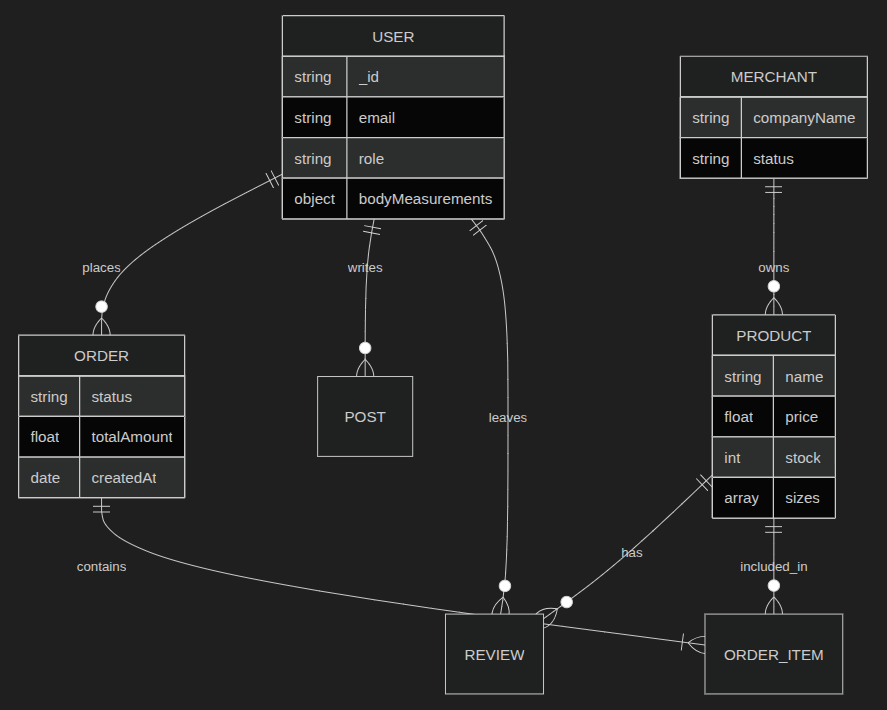
\includegraphics[width=\textwidth]{figures/erd.png}
    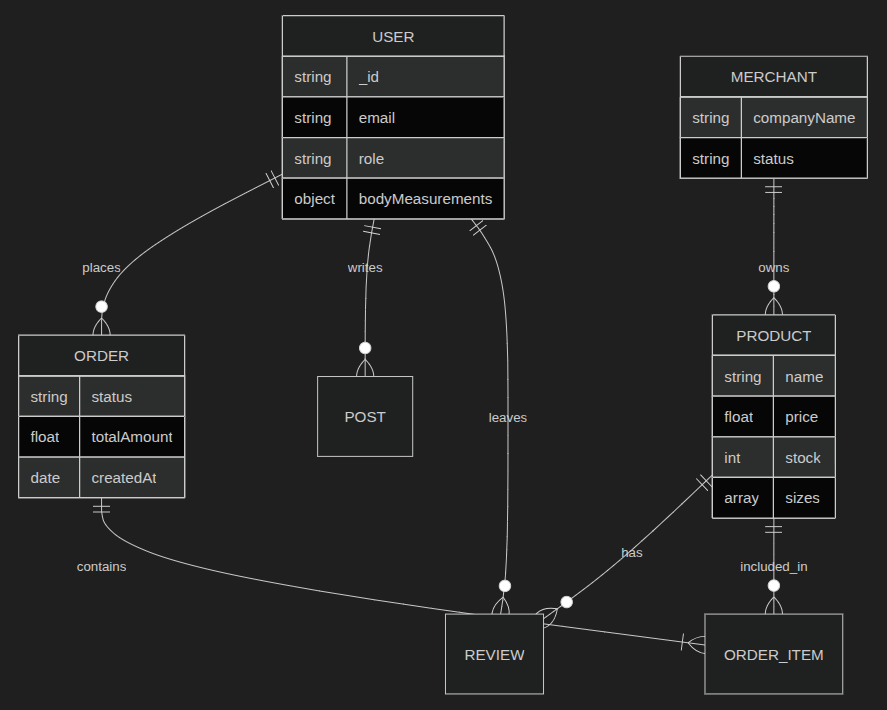
\includegraphics[width=\textwidth]{figures/erd.png}
    \caption{Entity-relationship diagram for \projectname.}
    \label{fig:erd}
\end{figure}

\subsection{Core Entities}

\textbf{User.} The central entity representing all platform users. Key attributes include name, email (with normalized duplicate), password (hashed, select-excluded), phone, address, birth date, role (user/merchant/admin/cs/designer), authentication provider (local/Google), profile images, body measurement fields (height\_cm, weight\_kg), a dedicated try-on image, account status flags (isActive, isSuspended), social counters (followersCount, followingCount), session tracking, and token management fields (tokenVersion, refreshToken, resetOTP).

\textbf{Product.} Represents a marketplace listing. Key attributes include name, description, price, sale price, stock count, merchant reference, category, garment type, image URLs, tags, available sizes, a size measurement chart (array of size-to-measurement mappings for chest, waist, hip, shoulder, inseam), colors, gender, material, brand, styles, occasions, and view count. Products are indexed on category, type, brand, price, merchant, tags, colors, and a text index on name, description, and brand for full-text search.

\textbf{Order.} Captures a purchase transaction. Contains a user reference, an array of order items (each with product reference, quantity, price, selected size, and selected color), total amount, status, delivery address, and payment method.

\textbf{MerchantProfile.} Extends a user with merchant-specific data: company name, company ID, national ID, and a list of product references.

\textbf{Review.} A product review containing user reference, product reference, rating (0.5--5), comment text, likes (array of user references), and threaded replies.

\textbf{TryOnResult.} Records a virtual try-on session. Contains user and product references, model type (vton2d/prova-vton/multiangle), result image URL and public ID, video generation status and metadata, garment category, and timestamps.

\textbf{BodyMeasurements.} Stores measurement estimation results. Contains user reference, engine used (shapy), source image URLs, input metadata (height, weight, gender, region, fit), the full measurements object, size recommendation, confidence scores, debug information, and processing time.

\subsection{Community Entities}

\textbf{Post.} A community post with author reference, type (issue/review/tip/question), title, content, optional images, optional store reference, optional rating, engagement counters (likesCount, commentsCount), and active status.

\textbf{Design.} A designer submission with name, description, category, price, designer reference, approval status (pending/approved/in\_production/published/rejected), vote counters, admin notes, and a computed virtual field for net votes.

\textbf{Comment.} A polymorphic comment that targets either a post or a design (via targetType and targetId). Supports threaded replies through a parentId self-reference. Tracks likesCount and repliesCount.

\textbf{Vote.} A polymorphic vote entity targeting posts, designs, or comments. Each vote has a type (like/upvote/downvote) and is uniquely constrained per user per target.

\textbf{Follow.} Represents a follower--following relationship between two users with a unique constraint preventing duplicate follows and a pre-save hook preventing self-follows.

\textbf{Notification.} Event-driven notifications with recipient, sender, type (like\_post, comment\_post, upvote\_design, follow, etc.), target reference, message text, read status, and a 30-day TTL auto-expiry index.

\textbf{Wishlist.} A polymorphic bookmark entity allowing users to save products, posts, or designs with optional notes. Uniquely constrained per user per item type and ID.

\textbf{SupportTicket.} Represents a customer service interaction. Contains user reference and contact details, optional agent assignment, status (open/assigned/resolved/closed), subject, priority (low/medium/high), a threaded messages array (each message with sender ID, name, role, content, and timestamp), last message preview, and unread counters for both user and agent sides.

\textbf{CustomerServiceProfile.} Extends a user with the customer service role. Links the agent to a specific branch for organizational routing.

\subsection{Key Relationships}
\begin{itemize}[leftmargin=*]
    \item A \textbf{User} has zero or more \textbf{Orders}, \textbf{Reviews}, \textbf{TryOnResults}, \textbf{BodyMeasurements}, \textbf{Posts}, \textbf{Designs}, \textbf{Comments}, \textbf{Votes}, \textbf{Wishlists}, and \textbf{Notifications}.
    \item A \textbf{Merchant} (User with merchant role) has one \textbf{MerchantProfile} and zero or more \textbf{Products}.
    \item A \textbf{Product} belongs to one \textbf{Merchant} and has zero or more \textbf{Reviews} and \textbf{OrderItems}.
    \item An \textbf{Order} belongs to one \textbf{User} and contains one or more \textbf{OrderItems}, each referencing a \textbf{Product}.
    \item A \textbf{Comment} belongs to one \textbf{User} and targets one \textbf{Post} or \textbf{Design}. Comments may have a parent \textbf{Comment} for threading.
    \item A \textbf{Vote} belongs to one \textbf{User} and targets one \textbf{Post}, \textbf{Design}, or \textbf{Comment}.
    \item A \textbf{Follow} connects two \textbf{Users} (follower and following).
\end{itemize}

\section{Class Diagram}

The class diagram illustrates the major software components and their relationships across the backend and AI services.

\begin{figure}[H]
    \centering
    % \includegraphics[width=\textwidth]{figures/class-diagram.png}
    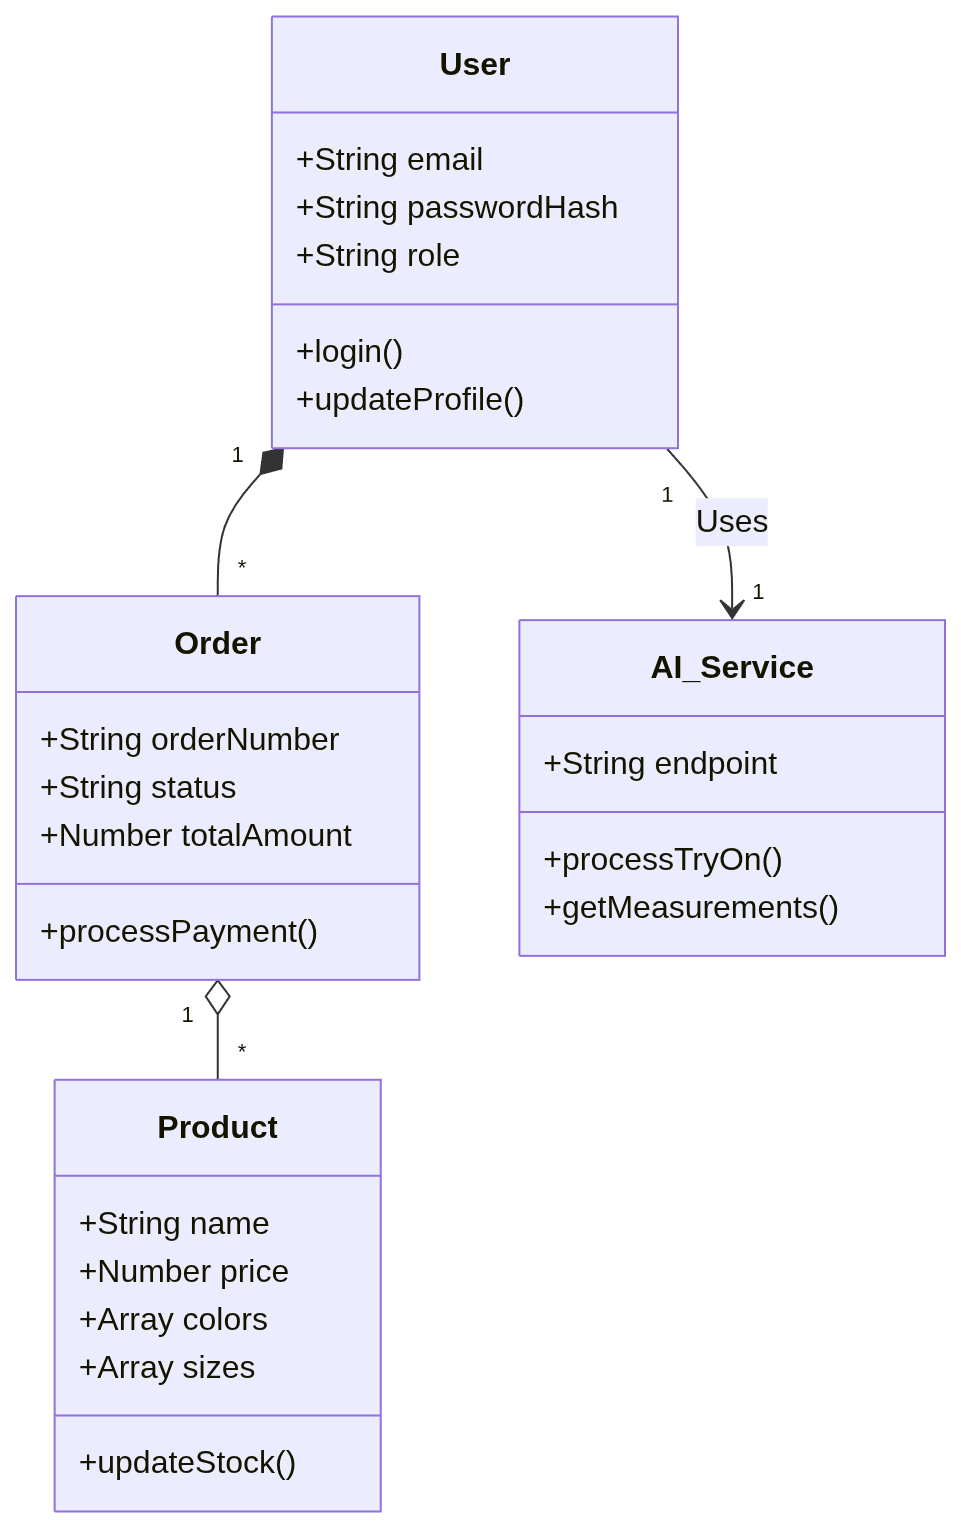
\includegraphics[width=\textwidth]{figures/classdiagram.png}
    \caption{Class diagram showing major components of \projectname.}
    \label{fig:classdiagram}
\end{figure}

The backend follows a layered module pattern. Each domain module (auth, product, order, post, etc.) contains four components: a \textbf{Routes} file that defines HTTP endpoints and attaches middleware, a \textbf{Controller} that handles request parsing and response formatting, a \textbf{Service} that implements business logic, and a \textbf{Model} that defines the Mongoose schema and database interface. Validation is handled by \textbf{Schema} files using Zod. Cross-cutting concerns—authentication, rate limiting, CORS, security headers, logging, and error handling—are implemented as Express middleware.

The try-on service follows a similar layered pattern using FastAPI. \textbf{Routers} define API endpoints, \textbf{Services} (ColabClient, MultiAngleClient, MultiviewClient, SHAPYClient, VideoPreprocessor) implement the AI pipeline logic, and \textbf{Models} define request/response schemas using Pydantic. A \textbf{Dependencies} module provides dependency injection for service instances, and a centralized \textbf{ClientState} singleton manages the lifecycle of all external service clients.

The RAG service is organized as a pipeline of composable stages: MessageClassifier, IntentExtractor, ProductRetriever, OutfitAssembler, and ResponseComposer, coordinated by a Pipeline orchestrator. Configuration, embeddings, prompts, and schemas are separated into dedicated modules.

\section{Process and Sequence Diagrams}

This section documents the key processes in the system using sequence diagrams that trace the flow of data and control across service boundaries.

\subsection{Product Purchase Flow}
\begin{figure}[H]
    \centering
    % 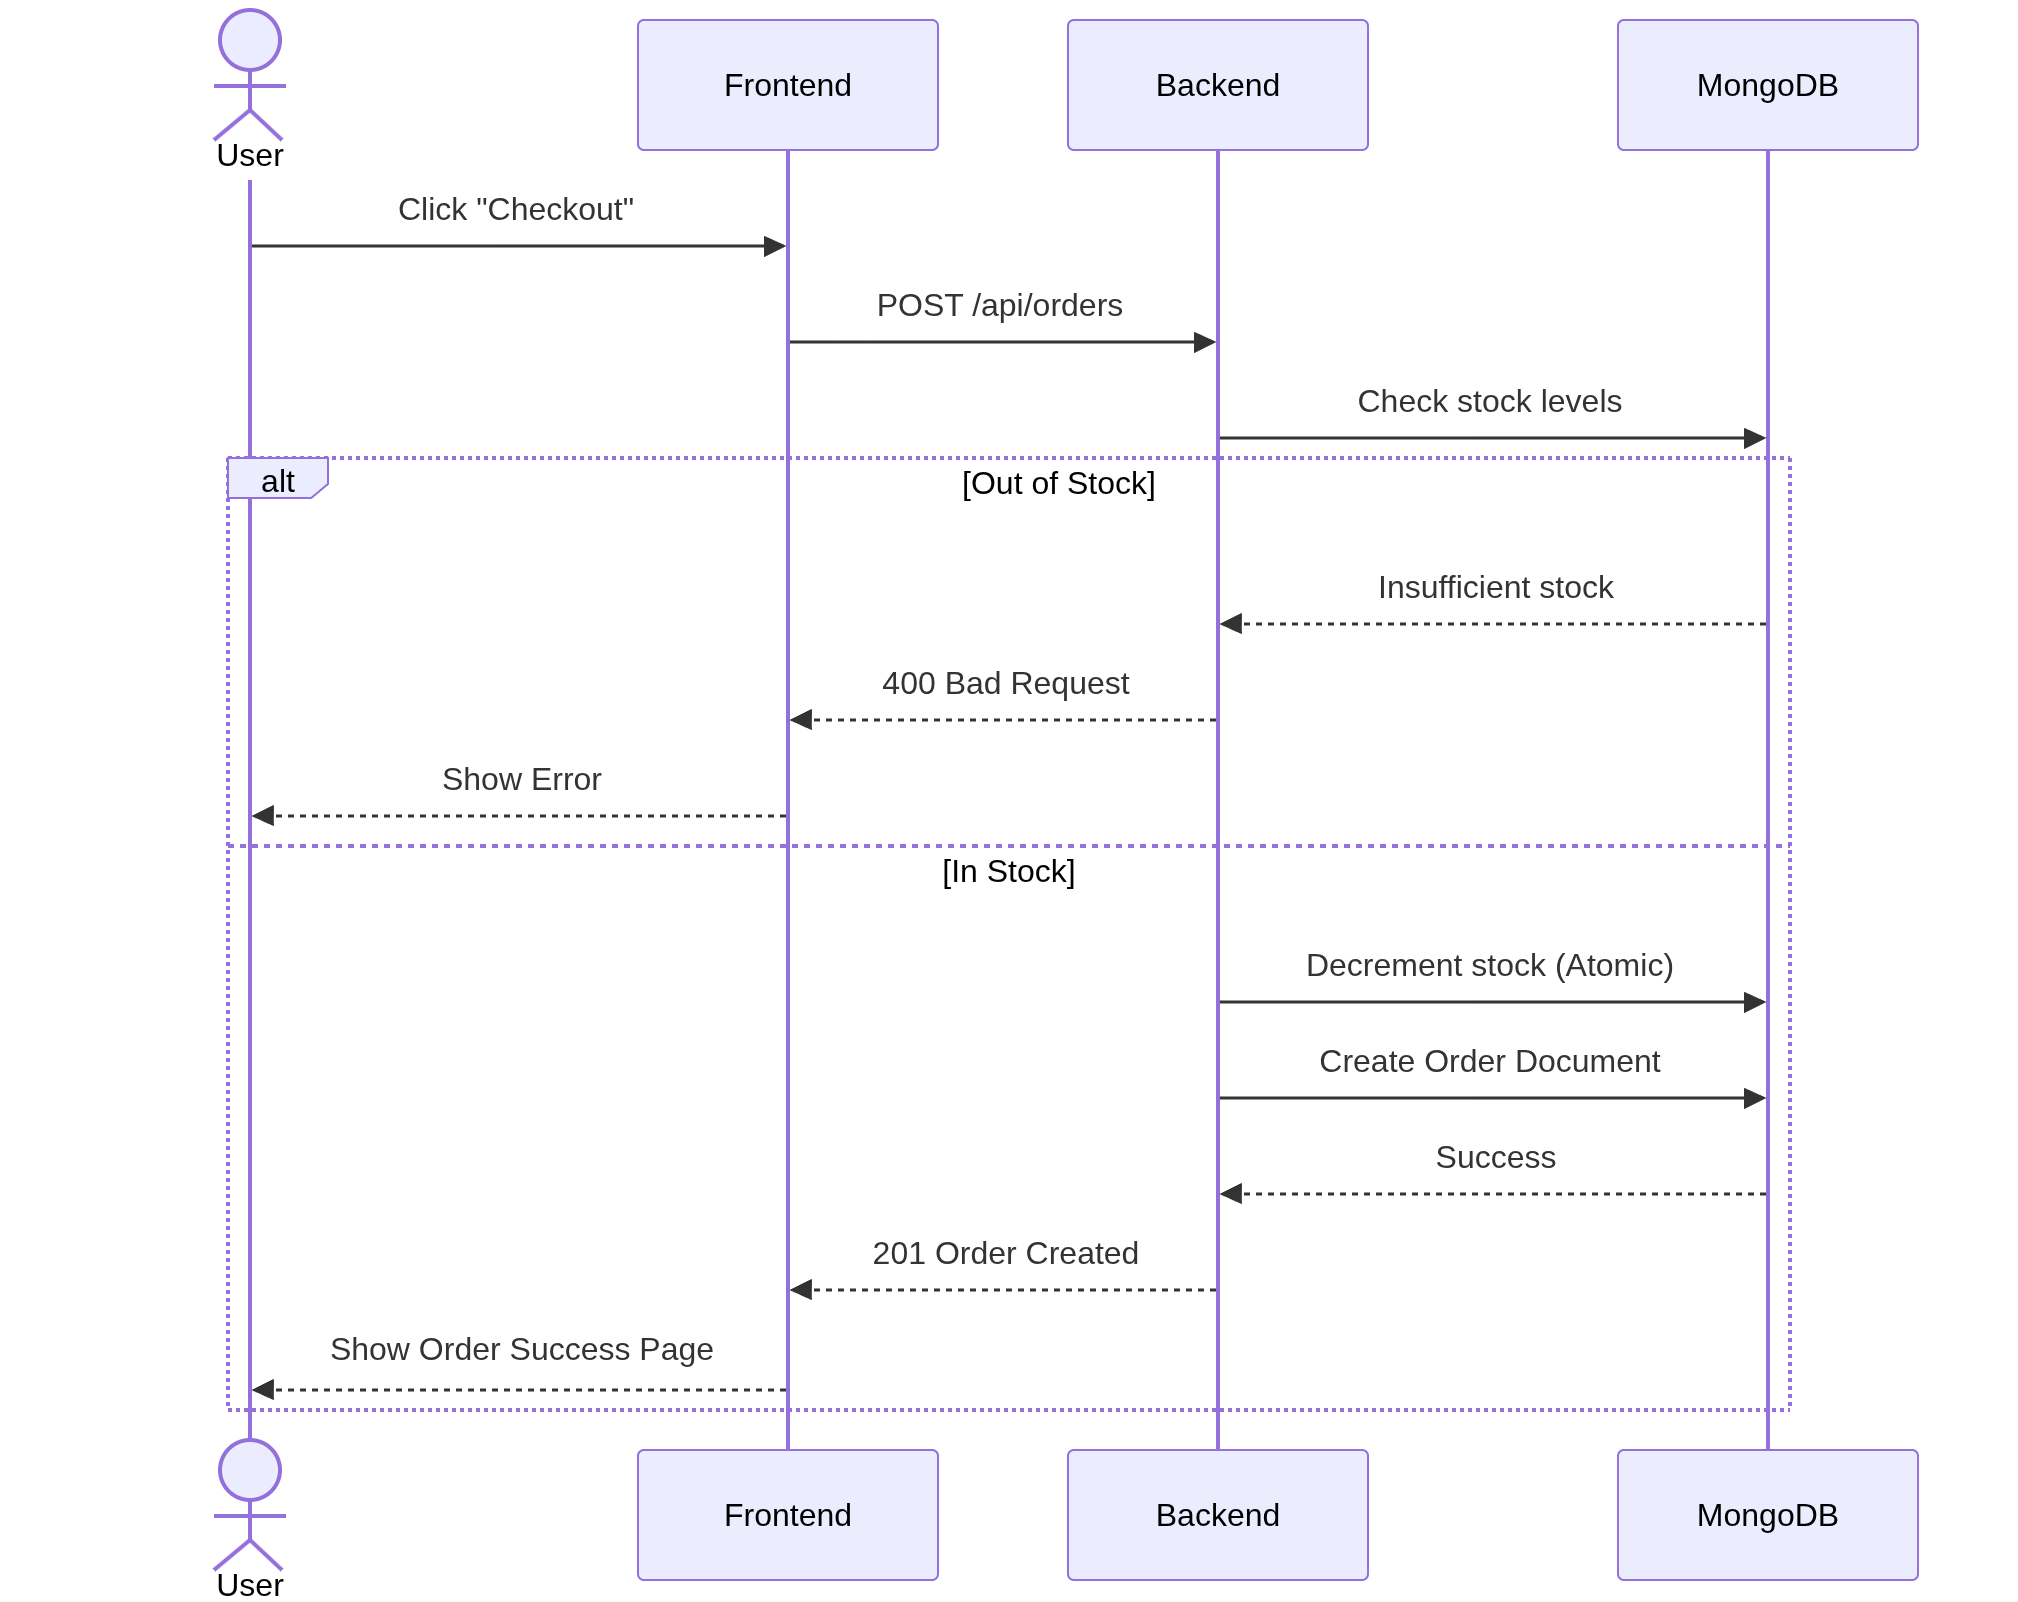
\includegraphics[width=\textwidth]{figures/seq-purchase.png}
    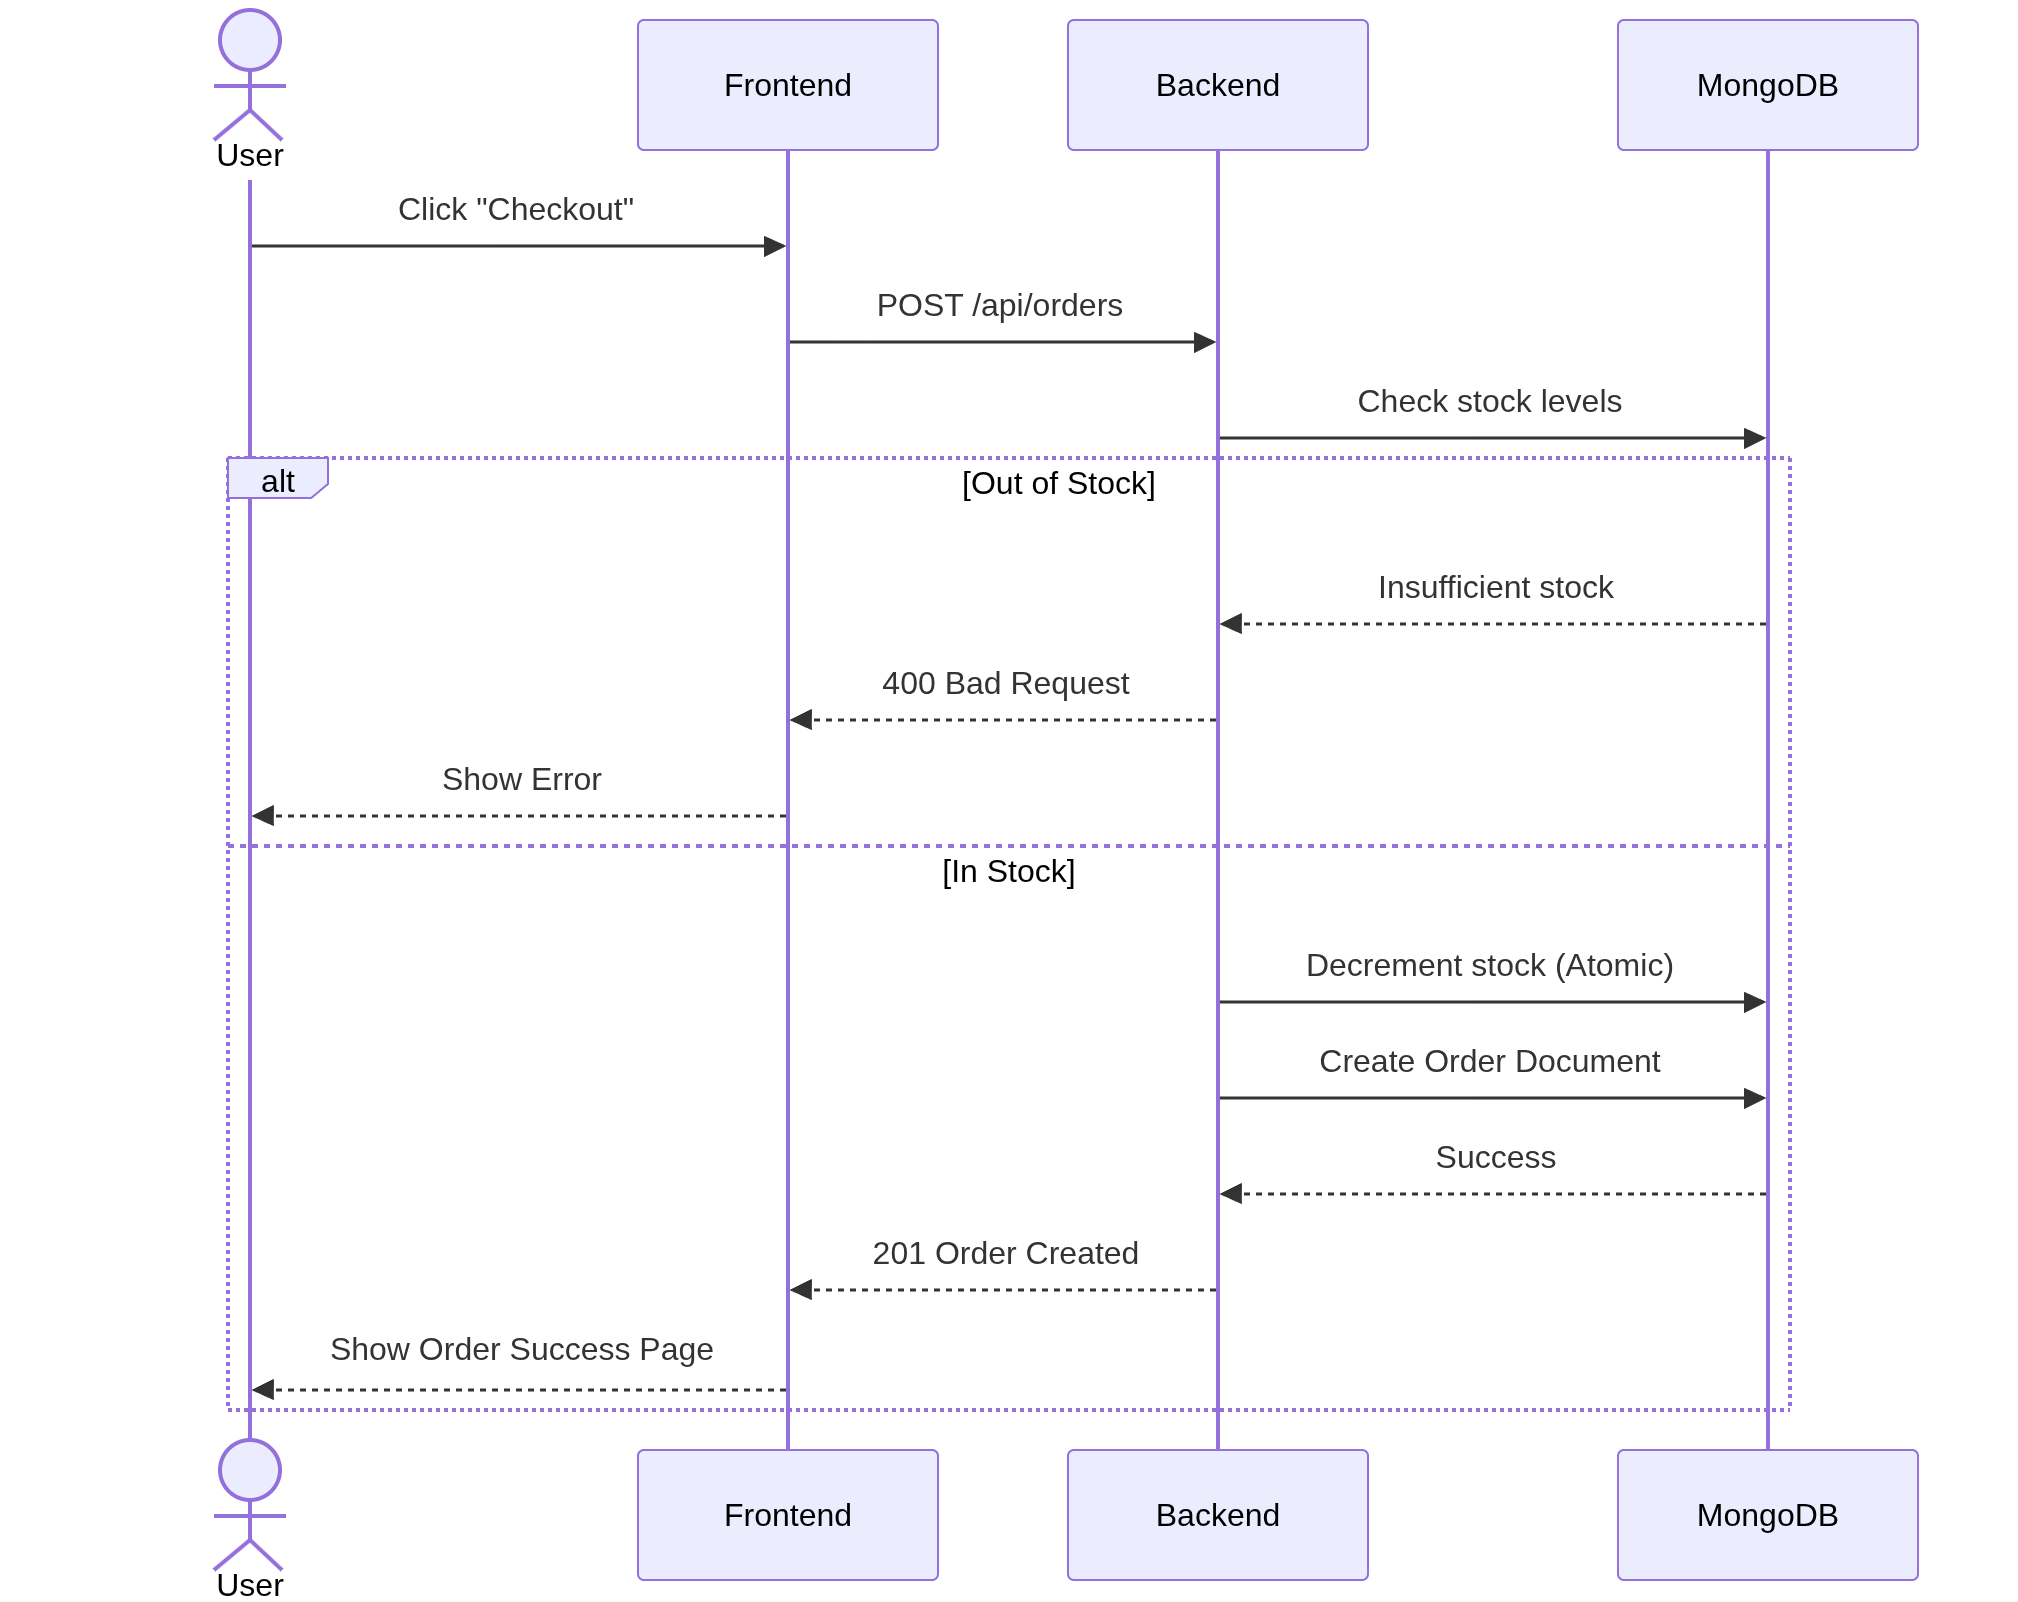
\includegraphics[width=0.9\textwidth]{figures/seq-purchase.png}
    \caption{Sequence diagram for the product purchase flow.}
    \label{fig:seq-purchase}
\end{figure}

The purchase flow proceeds as follows: (1) the shopper adds items to their cart on the frontend, (2) at checkout, the frontend sends a POST request to the backend order endpoint with items, address, and payment method, (3) the backend validates stock availability for each item, (4) the backend creates the order document and decrements stock for each product atomically, (5) the backend returns the order confirmation to the frontend, and (6) the frontend navigates to the order success page. If any item is out of stock, the backend returns a validation error before creating the order.

\subsection{Virtual Try-On Flow}
\begin{figure}[H]
    \centering
    % \includegraphics[width=\textwidth]{figures/seq-tryon.png}
    \includegraphics[width=0.9\textwidth]{figures/seq-tryon.png}
    \caption{Sequence diagram for the 2D virtual try-on flow.}
    \label{fig:seq-tryon}
\end{figure}

The 2D try-on flow involves three services: (1) the frontend uploads person and garment images to the backend, (2) the backend proxies the request to the try-on FastAPI service, (3) the try-on service validates and preprocesses both images, (4) the service sends the images to the custom trained diffusion model (Prova-VTON) for synthesis, (5) the result image is returned to the backend, (6) the backend uploads the result to cloud storage (Cloudinary), saves a TryOnResult document, and returns the image URL to the frontend.

\subsection{RAG Fashion Assistant Flow}
\begin{figure}[H]
    \centering
    % \includegraphics[width=\textwidth]{figures/seq-rag.png}
    \includegraphics[width=0.9\textwidth]{figures/seq-rag.png}
    \caption{Sequence diagram for the RAG fashion assistant pipeline.}
    \label{fig:seq-rag}
\end{figure}

The RAG flow proceeds through five stages: (1) the frontend sends the user's natural language message to the chat service, (2) the pipeline classifies the message intent—greetings and non-fashion queries receive immediate responses without retrieval, (3) for product searches, the intent extractor produces a structured query with attributes such as garment type, colors, and budget, (4) the retriever applies metadata filters against MongoDB and then ranks candidates by semantic similarity using Sentence-BERT embeddings, (5) the outfit assembler groups retrieved products into complete outfits, and (6) the response composer generates a bilingual explanation grounded in the actual retrieved products. The conversation turn is appended to the per-user history store for multi-turn context.

\subsection{Body Measurement Flow}
\begin{figure}[H]
    \centering
    % \includegraphics[width=\textwidth]{figures/seq-measurement.png}
    \includegraphics[width=0.9\textwidth]{figures/seq-measurement.png}
    \caption{Sequence diagram for body measurement and size recommendation.}
    \label{fig:seq-measurement}
\end{figure}

The measurement flow involves the following steps: (1) the frontend uploads a front-facing photograph along with height, weight, gender, and region parameters, (2) the backend forwards the request to the try-on service measurement endpoint, (3) the measurement router validates inputs and sends the image to the SHAPY service, (4) SHAPY performs 3D body mesh regression and returns raw shape parameters and circumference estimates, (5) the router applies weight-based circumference correction if the predicted mass deviates significantly from the user-provided weight, (6) derived measurements (widths, lengths) are computed using ISO 7250 anthropometric ratios, (7) the size recommendation module maps chest and waist circumferences to regional size charts with the selected fit preference, and (8) the complete result is returned with confidence scores and persisted to the database.

\subsection{Multiview Try-On and 360 Reconstruction Flow}

The multiview pipeline is the most complex workflow in the system and involves multiple stages across services: (1) the user uploads a video or set of images showing themselves from multiple angles, (2) the preprocessing service extracts frames (if video), runs person detection (YOLOv8), generates DensePose maps, and produces human parsing masks for each frame, (3) the user uploads garment front and back images, which are saved and organized, (4) the system builds a structured dataset ZIP containing the preprocessed person data and cloth images, (5) the ZIP is uploaded to the inference server, (6) the multiview try-on model generates view-consistent results across all viewpoints, (7) results are downloaded and extracted locally, and (8) the multiview outputs can be fed into the Splatfacto Gaussian splatting pipeline to produce an interactive 360-degree reconstruction.

\section{Summary}
This chapter has defined the functional and non-functional requirements for \projectname, identified the stakeholders and their interactions through use cases, documented the data model through entity descriptions and relationships, outlined the software architecture through a class diagram, and traced the key system processes through sequence diagrams. These analysis artifacts establish the foundation for the system design presented in Chapter~4 and the implementation details described in Chapter~5.

\chapter{Proposed System Design}

\section{Overview}
This chapter translates the requirements and analysis artifacts from Chapter~3 into concrete design decisions. It describes the high-level architecture, the internal structure of each service, the API design contracts, the data flow between services, the algorithmic stages within each AI pipeline, the security architecture, and the deployment topology. The design prioritizes modularity, independent scalability of AI workloads, and a clear separation between business logic and inference-heavy components.

\section{Architecture Overview}

\projectname\ follows a \textbf{service-oriented architecture (SOA)} comprising four independently deployable services that communicate over HTTP/REST:

\begin{enumerate}[leftmargin=*]
    \item \textbf{Frontend Service} — A Next.js application that renders the user interface, manages client-side state, handles internationalization (Arabic/English with RTL support), and communicates with the backend and AI services via REST calls.

    \item \textbf{Backend Service} — An Express.js application written in TypeScript that serves as the central orchestrator. It handles authentication, authorization, business logic for e-commerce and community features, proxies requests to AI services, and manages all persistent data through MongoDB.

    \item \textbf{Try-On Service} — A FastAPI application that exposes specialized endpoints for virtual try-on (2D and multiview), body measurement estimation, video preprocessing, and 360-degree reconstruction. It manages connections to external inference servers and local preprocessing pipelines.

    \item \textbf{Chat Service (RAG)} — A FastAPI application that implements the fashion-aware retrieval-augmented generation pipeline. It handles message classification, intent extraction, product retrieval with hybrid search, outfit assembly, and bilingual response generation.
\end{enumerate}

\begin{figure}[H]
    \centering
    \makebox[\textwidth][c]{\includegraphics[width=1.15\textwidth]{figures/arch-overview.png}}
    \caption{High-level service-oriented architecture of \projectname.}
    \label{fig:arch-overview}
\end{figure}

The frontend communicates directly with the backend for all e-commerce, authentication, and community operations. For AI features, two patterns are used: (1)~the backend proxies try-on and measurement requests to the Try-On Service, adding authentication validation and result persistence before forwarding; (2)~the frontend communicates directly with the Chat Service for real-time conversational interactions, as the RAG pipeline maintains its own in-memory conversation history and does not require backend-mediated persistence for the chat flow itself.

\section{Frontend Design}

\subsection{Framework and Routing}
The frontend uses \textbf{Next.js} with the App Router architecture. All user-facing pages are nested under a \texttt{[locale]} dynamic segment that enables locale-based routing. The locale parameter drives language selection (Arabic or English) and layout direction (RTL or LTR). The routing hierarchy is structured as follows:

\begin{verbatim}
app/
  [locale]/
    page.tsx              # Landing / Home
    shop/                 # Product catalog
    product/[id]/         # Product detail
    cart/                 # Shopping cart
    checkout/             # Checkout flow
    orders/               # Order history
    order-success/        # Order confirmation
    profile/              # User profile & settings
    virtual-tryon/        # Try-on interface
    community/            # Posts, designs, feed
    recommendations/      # AI-powered suggestions
    customer-service/     # Support ticket interface
    merchant-owner/       # Merchant dashboard
    admin/                # Admin panel
    login/ | signup/      # Authentication pages
    wishlist/             # Saved items
    dashboard/            # User dashboard
\end{verbatim}

\subsection{State Management and API Communication}
The frontend uses React hooks and context for local state management. API communication is centralized through a typed API client module that handles:
\begin{itemize}[leftmargin=*]
    \item Attaching JWT access tokens from local storage to all authenticated requests.
    \item Intercepting \texttt{401 Unauthorized} responses and checking for a refreshed token in the \texttt{X-New-Access-Token} response header (transparent token rotation).
    \item Providing typed request/response wrappers for each backend endpoint.
\end{itemize}

\subsection{Internationalization (i18n)}
The application supports Arabic and English through Next.js internationalized routing. Each locale has its own translation files loaded at build time. The layout component reads the current locale parameter and applies the appropriate \texttt{dir} attribute (\texttt{rtl} for Arabic, \texttt{ltr} for English) to the root HTML element. All UI text, labels, and messages reference translation keys rather than hardcoded strings.

\section{Backend Design}

\subsection{Module Architecture}
The backend follows a \textbf{layered module pattern} where each domain feature is encapsulated in its own directory under \texttt{src/modules/}. Every module contains four standard files:

\begin{itemize}[leftmargin=*]
    \item \textbf{Routes} (\texttt{*.routes.ts}) — Defines Express router endpoints, attaches middleware (authentication, validation, rate limiting), and maps HTTP methods to controller functions.
    \item \textbf{Controller} (\texttt{*.controller.ts}) — Parses request parameters and body, delegates to the service layer, and formats HTTP responses.
    \item \textbf{Service} (\texttt{*.service.ts}) — Contains business logic, database queries, and integration calls. Services are stateless functions.
    \item \textbf{Model} (\texttt{*.model.ts}) — Defines the Mongoose schema, TypeScript interfaces, indexes, and virtual fields for the module's data entity.
\end{itemize}

An optional \textbf{Schema} file (\texttt{*.schema.ts}) defines Zod validation schemas that are enforced by a generic validation middleware before the request reaches the controller.

\subsection{Middleware Pipeline}
Incoming requests pass through a layered middleware pipeline before reaching route handlers:

\begin{enumerate}[leftmargin=*]
    \item \textbf{Security Headers} — Helmet middleware applies HTTP security headers (Content-Security-Policy, X-Frame-Options, etc.).
    \item \textbf{CORS} — Configured to allow requests only from authorized frontend origins with credentials support.
    \item \textbf{Rate Limiting} — Two tiers: a general API rate limiter and a stricter authentication-specific rate limiter for login, signup, and password reset endpoints.
    \item \textbf{Body Parsing} — JSON and URL-encoded body parsing with configurable size limits.
    \item \textbf{Authentication} — JWT verification with automatic token refresh. The middleware extracts the Bearer token, verifies it against the JWT secret, and attaches the decoded user object to the request. If the access token is expired but a valid refresh token cookie is present, the middleware silently issues a new access token via the \texttt{X-New-Access-Token} response header.
    \item \textbf{Role Authorization} — A configurable role guard that checks whether the authenticated user's role is in the set of permitted roles for the endpoint.
    \item \textbf{Validation} — Zod schema validation middleware that validates request body, query, and params against the module's schema definitions, returning structured error responses on failure.
    \item \textbf{Profanity Guard} — Content moderation middleware applied to user-generated content endpoints.
\end{enumerate}

An \textbf{optional authentication middleware} variant is also provided for endpoints that enhance the experience for authenticated users but remain accessible to anonymous visitors (e.g., product browsing with personalized recommendations).

\subsection{User Caching}
To reduce database load on the authentication hot path, the backend implements an in-memory user cache. On successful JWT verification, the user document is stored in a TTL-bounded LRU cache keyed by user ID. Subsequent requests from the same user within the TTL window are served from cache, bypassing the MongoDB query. Cache entries are invalidated when the user's token version changes (e.g., after password change or forced logout).

\subsection{Error Handling}
A global error handler middleware catches all unhandled exceptions and returns standardized JSON error responses with appropriate HTTP status codes. Domain-specific errors (e.g., \texttt{ServiceUnavailableError}, \texttt{ExternalAPIError}, \texttt{ProcessingError}) are defined as custom exception classes that carry structured metadata for debugging.

\section{Try-On Service Design}

\subsection{Service Architecture}
The Try-On Service is a \textbf{FastAPI} application organized into routers, service clients, preprocessing modules, and a centralized dependency injection container.

\textbf{Routers} define the API surface:
\begin{itemize}[leftmargin=*]
    \item \texttt{/api/tryon} — Single-view 2D virtual try-on using Prova-VTON via a remote inference server.
    \item \texttt{/api/multiangle} — Multi-angle try-on using a multimodal generative model for front, right, left, and back viewpoints.
    \item \texttt{/api/prova-vton} — Multiview pipeline with preprocessing, dataset construction, remote inference, and result retrieval.
    \item \texttt{/api/measurements} — Body measurement estimation using the SHAPY client with size recommendation mapping.
    \item \texttt{/api/video360} — 360-degree video generation from multiview try-on outputs.
    \item \texttt{/api/health} — Aggregated health check across all service clients.
\end{itemize}

\textbf{Service Clients} encapsulate communication with external inference services. Each client follows a consistent pattern:
\begin{itemize}[leftmargin=*]
    \item Configurable base URL, timeouts, and connection pool limits via environment variables.
    \item Automatic retry with exponential backoff for transient failures (HTTP 429, 5xx).
    \item Health check methods for proactive monitoring.
    \item Structured exception hierarchy (\texttt{ServiceUnavailableError}, \texttt{ExternalAPIError}).
\end{itemize}

A \textbf{ClientState} singleton manages the lifecycle of all service clients. It is initialized once at application startup and provides dependency injection to routers via FastAPI's dependency system.

\subsection{Prova-VTON Model Training Architecture}
\label{sec:prova-vton-training-architecture}

The core of the try-on capabilities is powered by Prova-VTON, a custom diffusion-based generative model trained to synthesize realistic garment transfer under pose, appearance, and camera-view constraints. Figure~\ref{fig:vton-model-arch} shows the overall VTON training pipeline. The architecture receives six principal inputs: the target person image \(I_{target}\), the target pose map \(I_{pose}\), an agnostic person image \(I_{agnostic}\), a reference front garment image \(I_{ref\_front}\), a reference back garment image \(I_{ref\_back}\), and camera parameters such as rotation, translation, and intrinsic calibration values. These inputs jointly define what the model should reconstruct during training, which body geometry should be preserved, which visible clothing regions should be replaced, which garment appearance should be transferred, and from which viewpoint the final result should be generated.

\begin{figure}[H]
    \centering
    \makebox[\textwidth][c]{\includegraphics[width=1.15\textwidth]{figures/vton-model-arch.png}}
    \caption{Diffusion-based Prova-VTON training architecture with latent encoding, reference conditioning, pose guidance, camera conditioning, and denoising supervision.}
    \label{fig:vton-model-arch}
\end{figure}

\subsubsection*{Overall Pipeline Overview}
During training, the target image is treated as the reconstruction objective, while the agnostic image, pose map, reference garments, and camera parameters act as conditioning signals. The target image provides the ground-truth visual distribution that the diffusion model must learn to recover after noise is applied in latent space. The agnostic image removes or masks the original garment region from the person, allowing the model to preserve identity, body shape, hair, and background while avoiding direct copying of the original clothing. The pose map contributes structural information about body configuration, and the two reference garment images provide complementary appearance evidence for both front-facing and back-facing garment details. Camera parameters are included because multiview try-on requires the model to understand viewpoint-dependent appearance rather than generating each angle as an unrelated 2D image.

The data flow begins by encoding the target and agnostic images into latent representations. Noise is injected into the target latent at a randomly sampled diffusion timestep. In parallel, the pose map is processed by a PoseGuider, the garment references are encoded by CLIP and ReferenceNet modules, and the camera parameters are projected into a dense camera embedding. The denoising UNet then receives the noisy target latent concatenated with the agnostic latent, resulting in an 8-channel latent input. The conditioning features are injected into the denoising process through attention and feature-control mechanisms. The network is trained to predict the exact Gaussian noise that was added to the clean latent, which allows the reverse diffusion process to reconstruct a clean try-on latent during inference.

\subsubsection*{Latent Space Encoding}
Prova-VTON follows the latent diffusion paradigm. Instead of applying diffusion directly to high-resolution RGB pixels, a variational autoencoder (VAE) encoder \(E(\cdot)\) maps images into a compressed latent space. For the target image, the latent representation is defined as:

\begin{equation}
z = E(I_{target})
\end{equation}

where \(I_{target}\) is the ground-truth target image and \(z\) is its compact latent representation. The agnostic image is encoded in the same latent space to obtain \(z_{agnostic} = E(I_{agnostic})\). The VAE decoder \(D(\cdot)\) is used after denoising to transform the generated latent back into the image domain. Latent diffusion is used because it substantially reduces memory consumption and computational cost compared with pixel-space diffusion. This is particularly important for virtual try-on, where high-resolution garment textures, human body structure, and multiview consistency must be modeled simultaneously. The latent space also provides a more semantically organized representation, enabling the denoising network to focus on garment placement and appearance synthesis rather than low-level pixel reconstruction alone.

\subsubsection*{Reference Feature Extraction}
The reference branch is responsible for preserving garment identity. A CLIP-based reference encoder converts \(I_{ref\_front}\) and \(I_{ref\_back}\) into embedding vectors that capture high-level garment semantics, including category, silhouette, color, and texture cues. These embeddings are then further processed by ReferenceNet, an appearance encoder that produces spatial reference features suitable for injection into the denoising UNet. The use of both front and back garment images is important for multiview training because a single product image cannot reliably represent garment regions that become visible from side or rear viewpoints.

Camera conditioning is computed by passing the camera parameters through an embedding module, implemented conceptually as a Fourier or multilayer-perceptron projection. The resulting vector \(c_{cam}\) allows the network to associate visual evidence with the requested viewpoint. This design reduces inconsistencies such as front-view textures appearing incorrectly in back-view outputs, because the denoiser receives an explicit representation of the camera pose.

\subsubsection*{Forward Diffusion Process}
Training uses a denoising diffusion probabilistic model (DDPM) scheduler. At each iteration, a timestep \(t\) is randomly sampled from the training diffusion horizon, and Gaussian noise \(\epsilon\) is sampled from a standard normal distribution:

\begin{equation}
\epsilon \sim \mathcal{N}(0, I)
\end{equation}

The scheduler then produces a noisy latent \(z_t\) according to:

\begin{equation}
z_t = \sqrt{\bar{\alpha}_t} z + \sqrt{1 - \bar{\alpha}_t}\epsilon
\end{equation}

In this equation, \(z\) is the clean latent representation of the target image, \(z_t\) is the noised latent at timestep \(t\), \(\epsilon\) is the Gaussian noise added to the latent, and \(\bar{\alpha}_t\) is the cumulative product of the scheduler's noise-retention coefficients up to timestep \(t\). Small values of \(t\) preserve much of the original signal, while larger values of \(t\) make the latent increasingly noisy. Random timestep sampling teaches the model to denoise from different corruption levels, which is necessary for the iterative reverse diffusion process used during inference.

\subsubsection*{Conditioning Modules}
The conditioning modules provide the denoising network with information that cannot be inferred from the noisy latent alone. The PoseGuider converts \(I_{pose}\) into pose features that encode body layout, limb orientation, and spatial correspondence between the person and the intended garment region. These generated pose features guide the model toward anatomically plausible garment placement and reduce artifacts around arms, torso boundaries, and self-occlusions.

ReferenceNet produces generated reference features from the front and back garment images. These features carry the garment's appearance and are responsible for preserving details such as fabric color, collar structure, sleeves, seams, logos, and texture patterns. The camera embedding provides viewpoint awareness, enabling the same garment to be synthesized consistently across different camera directions. Together, these conditioning signals separate the main factors of variation: pose defines where the garment should appear, reference features define what the garment should look like, and camera features define how it should be observed.

\subsubsection*{UNet Denoising Network}
The denoising backbone is a conditional UNet with an encoder-decoder structure, skip connections, and cross-attention blocks. Its input is formed by concatenating the noisy target latent \(z_t\) and the agnostic latent \(z_{agnostic}\) along the channel dimension. Since each latent contains four channels, the concatenated tensor forms an 8-channel input. This input design allows the model to compare the corrupted target representation with the preserved person context from the agnostic image. The encoder progressively extracts abstract features, the bottleneck integrates global conditioning, and the decoder reconstructs a noise prediction at the original latent resolution. Skip connections preserve spatial detail across scales, which is essential for maintaining face, hands, body boundaries, and garment edges.

Pose features, reference features, and camera embeddings are injected through attention blocks. In the cross-attention formulation, the UNet hidden states provide the queries, while conditioning features provide keys and values:

\begin{equation}
\operatorname{Attention}(Q,K,V) = \operatorname{Softmax}\left(\frac{QK^T}{\sqrt{d}}\right)V
\end{equation}

Here, \(Q\) represents query vectors derived from the current UNet feature maps, \(K\) represents key vectors derived from conditioning features, \(V\) represents value vectors containing the conditioning information to be integrated, and \(d\) is the key dimensionality used for normalization. In Prova-VTON, this means that each spatial region of the denoising feature map can selectively attend to pose structure, garment appearance, and camera context. For example, pixels corresponding to the upper torso can attend strongly to jacket texture features, while arm regions can attend more heavily to pose features to maintain correct sleeve alignment.

\subsubsection*{Reference Attention Mechanism}
The reference attention mechanism is implemented through a Reference Control Writer and a Reference Control Reader. During the reference pass, ReferenceNet extracts garment-aware features from the front and back reference images, and the writer stores these features in a control buffer associated with the attention layers. During the main denoising pass, the reader retrieves the stored features and supplies them to the UNet attention blocks. This separation allows the model to encode garment appearance once and reuse it throughout denoising, rather than forcing the UNet to infer garment identity only from a single global embedding.

This mechanism is important for preserving garment appearance. Direct concatenation of reference images would require the network to learn alignment and feature selection implicitly, which is difficult when garment and body poses differ. Reference attention instead allows the denoiser to retrieve appearance cues dynamically at multiple resolutions. As a result, fine-grained garment details can be maintained while still adapting the garment to the target pose and camera view.

\subsubsection*{Noise Prediction and Training Objective}
The UNet is trained to predict the injected noise:

\begin{equation}
\hat{\epsilon} = \operatorname{UNet}(z_t, z_{agnostic}, F_{pose}, F_{ref}, c_{cam}, t)
\end{equation}

where \(\hat{\epsilon}\) is the predicted noise, \(F_{pose}\) denotes pose features, \(F_{ref}\) denotes reference garment features, \(c_{cam}\) denotes the camera embedding, and \(t\) denotes the diffusion timestep. The training loss is the mean squared error between the true noise and the predicted noise:

\begin{equation}
L_{MSE} = \mathbb{E}\left[\lVert \epsilon - \hat{\epsilon} \rVert^2\right]
\end{equation}

By minimizing this objective, the model learns how to remove noise from latent representations while respecting the agnostic body context and all conditioning signals. Since the clean latent \(z\) corresponds to the target try-on image, accurate noise prediction implicitly teaches the network to reconstruct clean latent representations that contain the correct person identity, garment appearance, pose alignment, and camera viewpoint.

\subsubsection*{Training and Inference Separation}
The architecture distinguishes clearly between training and inference. During training, the target image is available and is used to produce \(z\), sample \(z_t\), and compute the supervised noise-prediction loss. The ground-truth noise \(\epsilon\) is known because it is sampled by the training algorithm. During inference, the target image and ground-truth noise are not available. Instead, the process begins from random Gaussian latent noise, and the trained UNet iteratively predicts and removes noise while conditioned on the user's agnostic image, pose map, garment references, and camera parameters. After the final reverse diffusion step, the VAE decoder maps the denoised latent into the final try-on image:

\begin{equation}
\hat{I}_{tryon} = D(\hat{z}_0)
\end{equation}

where \(\hat{z}_0\) is the final denoised latent and \(\hat{I}_{tryon}\) is the synthesized try-on output. This reconstruction stage converts the learned latent representation into a human-viewable image suitable for display in the e-commerce interface or for later use in multiview and 360-degree preview workflows.

\subsection{Multi-Angle Try-On Pipeline Design}
The multi-angle try-on client implements a two-stage pipeline for producing realistic virtual try-on results across multiple viewpoints:

\textbf{Stage 1 --- Garment Preparation.} Before try-on synthesis, the system determines whether the garment reference image contains a model wearing the garment or is a flat product shot. The decision is made through a three-step heuristic:
\begin{enumerate}[leftmargin=*]
    \item Check for transparent background (alpha channel analysis) --- transparent images are classified as flat product shots.
    \item Detect skin-tone pixels using RGB-space rules and check for portrait aspect ratio --- images with significant skin content in portrait orientation are classified as model-worn.
    \item If the source mode is ambiguous (\texttt{auto}), the heuristic result is used; explicit modes (\texttt{flat\_product}, \texttt{model\_worn}) override the heuristic.
\end{enumerate}

For model-worn garment references, an extraction step uses the multimodal model to isolate the garment from the person, producing a clean product image before try-on synthesis.

\textbf{Stage 2 --- Try-On Synthesis.} The prepared garment image and the person image are submitted to the generative model with a composed prompt. The prompt is dynamically constructed from a base template augmented with control parameters:
\begin{itemize}[leftmargin=*]
    \item \textbf{Garment type} (upper/lower/dress/shoes) --- instructs the model on which body region to modify.
    \item \textbf{Shirt placement} (tucked/untucked) --- controls hem behavior.
    \item \textbf{View hint} (front/right/left/back) --- preserves the camera orientation of the person image.
\end{itemize}

For multi-angle try-on, the system processes multiple viewpoints concurrently using an asyncio semaphore (concurrency limit of 2) to balance throughput against API rate limits. Garment preparation is performed once and shared across all views.

\subsection{Multiview (Prova-VTON) Pipeline Design}
The multiview pipeline is designed for generating view-consistent try-on results across all angles. It operates in five stages:

\begin{enumerate}[leftmargin=*]
    \item \textbf{Preprocessing} — Input video or images are processed through YOLOv8 for person detection, Detectron2 for DensePose map generation, and a human parsing network for segmentation masks. Results are organized into a structured directory hierarchy.

    \item \textbf{Cloth Preparation} — Garment front and back images are saved, resized, and organized into the dataset structure expected by the inference model.

    \item \textbf{Dataset Construction} — Person preprocessing outputs and cloth images are assembled into a ZIP archive following the model's expected directory format, ready for upload.

    \item \textbf{Remote Inference} — The ZIP is uploaded to the inference server. The service polls for job completion with configurable timeouts.

    \item \textbf{Result Retrieval} — Completed results are downloaded, extracted, and made available through the API. The multiview outputs can optionally be fed into the Splatfacto 3D Gaussian splatting pipeline for 360-degree interactive reconstruction.
\end{enumerate}

\begin{figure}[H]
\centering
\begin{tikzpicture}[
    node distance=1.5cm and 1cm,
    process/.style={rectangle, minimum width=3.5cm, minimum height=1cm, text centered, draw=provablue, fill=provalight, font=\small\bfseries, rounded corners},
    arrow/.style={thick,->,>=stealth, provablue}
]

% Nodes
\node (n1) [process] {1. Preprocessing (YOLO, DensePose, SCHP)};
\node (n2) [process, below=of n1] {2. Cloth Preparation (RGB/JPEG Format)};
\node (n3) [process, below=of n2] {3. Dataset Construction (ZIP Archive)};
\node (n4) [process, below=of n3] {4. Remote Inference (GPU Cluster)};
\node (n5) [process, below=of n4] {5. Result Retrieval \& 3D Splatting};

% Arrows
\draw [arrow] (n1) -- (n2);
\draw [arrow] (n2) -- (n3);
\draw [arrow] (n3) -- (n4);
\draw [arrow] (n4) -- (n5);

\end{tikzpicture}
\caption{The five-stage architecture of the Prova-VTON multiview pipeline.}
\label{fig:prova-vton-pipeline}
\end{figure}

\subsection{Measurement Pipeline Design}
The measurement pipeline transforms a single front-facing photograph into body measurements and size recommendations through the following stages:

\begin{enumerate}[leftmargin=*]
    \item \textbf{Input Validation} — The router validates image format, file size, height (in cm), weight (in kg), and gender parameters.

    \item \textbf{SHAPY Inference} — The image and metadata are sent to the SHAPY service, which performs SMPL-X body mesh regression and returns raw shape parameters and circumference estimates.

    \item \textbf{Weight-Based Correction} — If the predicted body mass deviates significantly from the user-provided weight, the router applies a proportional correction factor to circumference measurements. This compensates for the inherent ambiguity of estimating depth information from a single 2D image.

    \item \textbf{Derived Measurements} — Additional body dimensions (shoulder width, arm length, trouser length, thigh circumference) are computed from the corrected circumferences using ISO~7250 anthropometric ratios.

    \item \textbf{Size Recommendation} — Chest and waist circumferences are mapped to regional size charts (EU, US, UK, IT, FR, DE) with configurable fit preferences (regular, slim, oversized). The fit preference applies a scaling factor: slim reduces the target circumference, oversized increases it.

    \item \textbf{Confidence Scoring} — Each measurement receives a confidence score based on the quality of the input image, the magnitude of corrections applied, and the consistency between predicted and reported anthropometric data.
\end{enumerate}

\section{Chat Service (RAG) Design}

\subsection{Fashion Recommendation RAG Architecture}
\label{sec:rag-architecture}

The Chat Service implements a fashion recommendation architecture based on retrieval-augmented generation. Its purpose is to transform a user's natural language shopping request into grounded product and outfit recommendations drawn from the actual catalog. Figure~\ref{fig:rag-model-arch} shows the complete RAG recommendation workflow. The design separates retrieval from generation: retrieval identifies products that satisfy the user's constraints, while generation converts those retrieved products into a natural, bilingual explanation. This separation is essential in an e-commerce setting because the assistant must not merely produce plausible fashion advice; it must recommend items that exist in inventory and satisfy availability, category, price, style, and user-preference constraints.

\begin{figure}[H]
    \centering
    \makebox[\textwidth][c]{\includegraphics[width=1.15\textwidth]{figures/rag-model-arch.png}}
    \caption{Fashion recommendation RAG architecture from user message classification to hybrid retrieval, outfit scoring, bilingual response composition, and final output.}
    \label{fig:rag-model-arch}
\end{figure}

\subsubsection*{User Query Processing}
The workflow begins when the user submits a message through the AI fashion assistant. The Message Classifier determines whether the message is a product-search request, a greeting, a follow-up, a clarification, or a non-fashion query. This early decision prevents unnecessary retrieval for messages that do not require catalog access. For example, greetings and general conversational turns are routed to a Quick Response module, which returns a concise response without invoking the retrieval and ranking pipeline. Non-fashion messages are also handled through this fast path, keeping the assistant focused on the shopping domain.

When the classifier detects a product-search intent, the message is forwarded to the intent extraction stage. This creates a clear distinction between conversational inference and recommendation inference. Conversational inference handles lightweight replies, while recommendation inference performs structured interpretation, database retrieval, semantic ranking, outfit assembly, and response generation.

\subsubsection*{Intent Extraction}
The Intent Extractor converts natural language into a structured fashion intent. The extracted intent may include style, occasion, season, gender, garment type, colors, size, budget, brand preferences, fit, material, and additional attributes. For example, the message ``I need a modest summer outfit for a casual university day'' can be converted into an intent containing \texttt{style=modest}, \texttt{season=summer}, \texttt{occasion=casual/university}, \texttt{gender} inferred from the user profile when available, and relevant garment categories such as tops, trousers, and light outerwear. Similarly, ``Find me a black formal dress under 2000 EGP'' maps to a structured query with color, occasion, garment type, and price constraints.

This structured representation is necessary because product catalogs are not searched effectively by raw natural language alone. Hard constraints such as price range, size, gender, and stock availability must be represented explicitly so that retrieval does not return unsuitable products. At the same time, softer preferences such as ``elegant,'' ``streetwear,'' or ``minimal'' are preserved for semantic ranking because they may not correspond to exact database fields.

\subsubsection*{Hybrid Retrieval Layer}
The Hybrid Retriever combines MongoDB metadata filtering with semantic retrieval using Sentence-BERT. The first mechanism applies deterministic filters over catalog fields. MongoDB queries restrict the candidate set according to attributes such as category, gender, color, size availability, price range, brand, and stock status. This stage improves precision and computational efficiency by eliminating products that violate explicit user constraints before semantic ranking is performed.

The second mechanism ranks the remaining candidates using dense embeddings. The user's query is encoded as:

\begin{equation}
q = \operatorname{SBERT}(\operatorname{Query})
\end{equation}

Each product is represented by an embedding computed from its searchable textual fields:

\begin{equation}
p_i = \operatorname{SBERT}(\operatorname{Product}_i)
\end{equation}

The semantic relevance between the user query and product \(i\) is measured using cosine similarity:

\begin{equation}
\operatorname{Similarity}(q,p_i) = \frac{q \cdot p_i}{\lVert q \rVert \lVert p_i \rVert}
\end{equation}

Here, \(q\) is the query embedding, \(p_i\) is the embedding of the \(i\)-th product, \(q \cdot p_i\) is their dot product, and \(\lVert \cdot \rVert\) denotes vector magnitude. Cosine similarity is appropriate because it measures directional closeness in embedding space, allowing semantically related descriptions to match even when they do not share exact keywords. The hybrid design improves recommendation quality by combining the precision of structured filtering with the flexibility of semantic understanding.

\subsubsection*{Retrieval Phase}
The retrieval phase generates candidate products, ranks them, and selects the top products for outfit construction. Candidate generation begins with metadata filtering so that the system respects explicit constraints. Dense ranking then orders candidates according to semantic relevance. Products with low similarity can be discarded, while the highest-ranked products are passed forward as top candidate products. This staged design reduces hallucination risk because the response composer receives only verified catalog items rather than unconstrained model-generated suggestions.

\subsubsection*{Outfit Assembler}
The Outfit Assembler builds complete outfits from the retrieved items. Rather than recommending isolated products independently, the assembler groups items according to category compatibility and styling logic. For example, a top can be paired with trousers or a skirt, outerwear can be added when appropriate for the season, and shoes or accessories can be included when available. The assembler also avoids incompatible combinations, such as pairing two primary tops in the same outfit unless one is classified as an outer layer. This step translates product retrieval into a more useful fashion recommendation because users typically seek complete looks rather than disconnected catalog entries.

\subsubsection*{Outfit Scoring Engine}
After candidate outfits are assembled, a scoring engine evaluates them using a six-dimensional framework. The overall outfit score can be expressed as:

\begin{equation}
\operatorname{Score}(\operatorname{outfit}) = \sum_i w_i s_i
\end{equation}

In this equation, \(s_i\) is the score assigned to the outfit on dimension \(i\), and \(w_i\) is the weight expressing the importance of that dimension. Suitable dimensions include style compatibility, color harmony, occasion suitability, seasonal suitability, trend alignment, and user preference matching. Style compatibility measures whether the selected products belong to a coherent aesthetic. Color harmony checks whether the palette is visually consistent. Occasion suitability evaluates whether the outfit matches the intended use case, such as formal events, university, work, or casual wear. Seasonal suitability considers fabric weight, sleeve length, and layering. Trend alignment reflects current or catalog-defined fashion signals, while user preference matching incorporates profile information, previous conversation context, and explicit constraints.

The weighted formulation allows the system to adapt recommendations to different situations. For a wedding query, occasion suitability may receive a high weight; for a user asking for daily basics, comfort, color neutrality, and preference matching may become more important. The scoring engine therefore provides a principled way to rank outfits beyond simple product-level relevance.

\subsubsection*{Outfit Grouping and Ranking}
The grouped outfits are ranked according to their total scores and diversity constraints. Grouping similar outfits prevents the assistant from returning several near-identical combinations that differ only by minor product substitutions. Ranking then selects the best recommendations according to the scoring function, while diversity ensures that the final response contains meaningful alternatives. This step improves user experience by presenting a small set of strong, distinct recommendations rather than a long list of products.

\subsubsection*{Bilingual Response Composer}
The Bilingual Response Composer receives the selected outfits, product metadata, the original user query, conversation history, and available user profile information. It generates a human-readable response in English or Arabic, depending on the user's language preference or detected message language. The response is grounded in the retrieved products and includes explanations for why each outfit was selected. For instance, it may explain that a linen shirt was recommended because it matches a summer requirement, or that a darker trouser balances a bright top for a more formal appearance.

This generation stage is intentionally placed after retrieval and scoring. The language model is not responsible for inventing products; it is responsible for communicating catalog-grounded recommendations clearly. This design supports bilingual interaction while preserving factual alignment with the product database.

\subsubsection*{Final System Output}
The final output returned to the user consists of one or more recommended outfits, associated product references, and explanatory text. End-to-end, information moves from an unstructured user message to a classified intent, then to a structured fashion query, through hybrid retrieval, outfit assembly, scoring, grouping, and finally bilingual response generation. If the message is not a product-search request, the system bypasses the retrieval path and returns a quick response. If it is a product-search request, the full RAG workflow ensures that recommendations are relevant, available, stylistically coherent, and explainable.

\subsection{Conversation History}
The service maintains per-user conversation history in an in-memory LRU (Least Recently Used) store. The store is keyed by \texttt{user\_id} (primary) or \texttt{session\_id} (fallback), with configurable limits: up to 5{,}000 distinct keys and 20 turns (user + assistant messages) per key. Older entries are evicted when limits are reached. This enables multi-turn conversations where the assistant can reference previous queries without requiring external storage.

\subsection{Knowledge Base Integration}
A fashion-specific knowledge base provides profile-aware styling guidance. The knowledge base contains rules indexed by body type, height range, and gender that map to recommended silhouettes, colors, and fit preferences. When the user's profile includes height, weight, and gender, the retriever consults the knowledge base to augment recommendations with personalized styling advice.

\subsection{Embedding Strategy}
Product embeddings are pre-computed using Sentence-BERT (\texttt{all-MiniLM-L6-v2}) over a concatenation of product name, description, brand, tags, styles, and occasion fields. Embeddings are stored alongside product documents in MongoDB. A dedicated admin endpoint (\texttt{POST /precompute-embeddings}) triggers bulk re-computation when the product catalog is updated.

\section{API Design}

The system exposes RESTful APIs following consistent design conventions:

\subsection{Backend API Conventions}
\begin{itemize}[leftmargin=*]
    \item \textbf{URL Structure}: Resources follow a noun-based hierarchy (e.g., \texttt{/api/products}, \texttt{/api/orders/:id}, \texttt{/api/community/posts}).
    \item \textbf{Authentication}: Protected endpoints require a \texttt{Bearer} token in the \texttt{Authorization} header. Public endpoints use the optional auth middleware.
    \item \textbf{Response Format}: All responses follow a consistent JSON structure with \texttt{success} (boolean), \texttt{msg} (human-readable message), and \texttt{data} (payload) fields.
    \item \textbf{Error Format}: Errors include \texttt{success: false}, a machine-readable \texttt{code} (e.g., \texttt{TOKEN\_EXPIRED}), and a descriptive \texttt{msg}.
    \item \textbf{Pagination}: List endpoints support \texttt{page} and \texttt{limit} query parameters with default values.
    \item \textbf{Validation}: Request bodies are validated against Zod schemas before reaching controllers.
\end{itemize}

\subsection{Try-On Service API}
The Try-On Service accepts multipart form data for image uploads. Key endpoints include:

\begin{longtable}{l c p{8cm}}
\toprule
\textbf{Endpoint} & \textbf{Method} & \textbf{Description} \\
\midrule
\endfirsthead
\toprule
\textbf{Endpoint} & \textbf{Method} & \textbf{Description} \\
\midrule
\endhead
\bottomrule
\endfoot

\texttt{/api/tryon/try-on} & POST & Submit person and garment images for 2D try-on using Prova-VTON. \\
\texttt{/api/multiangle/tryon} & POST & Single-view try-on with garment type, source mode, and placement controls. \\
\texttt{/api/multiangle/multi} & POST & Multi-angle try-on across front, right, left, and back viewpoints. \\
\texttt{/api/measurements/measure} & POST & Body measurement estimation from a front-facing photograph. \\
\texttt{/api/prova-vton/preprocess} & POST & Preprocess person video/images for the multiview pipeline. \\
\texttt{/api/prova-vton/upload-cloth} & POST & Upload garment front and back images. \\
\texttt{/api/prova-vton/build-dataset} & POST & Assemble preprocessed data into inference-ready format. \\
\texttt{/api/prova-vton/infer} & POST & Submit dataset for multiview inference. \\
\texttt{/api/prova-vton/results} & GET & Retrieve completed inference results. \\
\texttt{/api/health} & GET & Aggregated health status across all service clients. \\
\end{longtable}

\subsection{Chat Service API}
\begin{longtable}{l c p{8cm}}
\toprule
\textbf{Endpoint} & \textbf{Method} & \textbf{Description} \\
\midrule
\endfirsthead
\toprule
\textbf{Endpoint} & \textbf{Method} & \textbf{Description} \\
\midrule
\endhead
\bottomrule
\endfoot

\texttt{/chat} & POST & Send a natural language message through the RAG pipeline. Accepts \texttt{message}, \texttt{userId}, \texttt{sessionId}, and \texttt{lang}. \\
\texttt{/health} & GET & Service health check with uptime reporting. \\
\texttt{/precompute-embeddings} & POST & Admin utility to re-compute all product embeddings. \\
\end{longtable}

\section{Security and Privacy Design}

\subsection{Authentication Flow}
The system implements a dual-token authentication strategy:
\begin{itemize}[leftmargin=*]
    \item \textbf{Access Token} — A short-lived JWT (configurable TTL, typically 15 minutes) containing \texttt{userId} and \texttt{tokenVersion}. Sent in the \texttt{Authorization: Bearer} header.
    \item \textbf{Refresh Token} — A longer-lived JWT stored as an HTTP-only cookie. Used to silently rotate access tokens when they expire.
    \item \textbf{Token Versioning} — Each user has a \texttt{tokenVersion} counter. Changing the password or performing a forced logout increments this version, immediately invalidating all existing tokens.
\end{itemize}

\subsection{Password Security}
Passwords are hashed using \textbf{bcrypt} with a configurable salt rounds parameter before storage. Raw passwords are never persisted or logged. The password field is excluded from all database queries by default using Mongoose's \texttt{select: false} option.

\subsection{Rate Limiting}
Two tiers of rate limiting protect the system:
\begin{itemize}[leftmargin=*]
    \item \textbf{General API rate limiter} — Applied to all endpoints with a generous window to prevent abuse while allowing normal usage patterns.
    \item \textbf{Authentication rate limiter} — Stricter limits on login, signup, and password reset endpoints to mitigate brute-force attacks. A separate \textbf{password reset rate limiter} is applied to the forgot-password, verify-code, and reset-password flow.
\end{itemize}

\subsection{Input Validation and Sanitization}
All user inputs are validated at two levels:
\begin{itemize}[leftmargin=*]
    \item \textbf{Schema validation} (Zod) — Ensures type safety, required fields, string length limits, and format constraints (e.g., email format, phone number patterns).
    \item \textbf{Content moderation} — A profanity guard middleware scans user-generated text content before it reaches the database.
\end{itemize}

\subsection{Data Privacy}
Uploaded images for try-on and body measurements are processed in-memory where possible and stored in Cloudinary with access-controlled URLs. Try-on results are associated with authenticated user accounts, ensuring that results are only accessible to the user who generated them. The body measurement pipeline does not retain raw images beyond the inference session unless explicitly saved by the user.

\section{Deployment Architecture}

The system is designed for deployment across multiple environments:

\begin{itemize}[leftmargin=*]
    \item \textbf{Frontend} — Deployed as a containerized Next.js application behind a reverse proxy (Nginx or Vercel). Static assets are served from a CDN.

    \item \textbf{Backend} — Runs as a Node.js process with PM2 for process management and automatic restarts. Connects to a managed MongoDB Atlas cluster.

    \item \textbf{Try-On Service} — Runs as a Uvicorn ASGI server. GPU-intensive inference (Prova-VTON) is offloaded to remote GPU servers accessed via HTTP. The local service handles preprocessing, orchestration, and result delivery.

    \item \textbf{Chat Service} — Runs as a Uvicorn ASGI server. The Sentence-BERT embedding model runs locally on CPU. LLM inference is delegated to an external API endpoint.

    \item \textbf{Database} — MongoDB Atlas provides the primary data store with automated backups, replica sets for high availability, and Atlas Search for text indexing.

    \item \textbf{Media Storage} — Cloudinary serves as the cloud media storage provider for product images, profile photos, try-on results, and community post images.
\end{itemize}

\section{Summary}
This chapter has presented the system design for \projectname, covering the service-oriented architecture, the internal design of each service (frontend routing and i18n, backend module pattern and middleware pipeline, try-on multi-stage pipelines, and RAG pipeline stages), the API contracts, the security architecture, and the deployment topology. These design decisions directly implement the requirements defined in Chapter~3 and provide the blueprint for the implementation described in Chapter~5.

\chapter{Implementation}

\section{Overview}
This chapter describes how \projectname\ is implemented across the frontend, backend, and AI services. It also documents the models, datasets, and results that validate the marketplace, RAG retrieval, multiview 2D try-on, measurement estimation, and 360 view features.

\section{Backend Implementation}
The backend is written in TypeScript using Express. It provides REST endpoints for authentication, product and order management, community content, and proxying AI requests. Validation is performed using schema-based checks, and MongoDB is used for persistence.

\section{Frontend Implementation}
The frontend uses Next.js with the App Router. It integrates localization, UI components, and interactive workflows for marketplace browsing, community engagement, designer pages, and 2D try-on.

\section{Try-On Service Implementation}
The FastAPI try-on service exposes endpoints for the custom multiview 2D try-on pipeline. The implementation follows the same high-level stages described in the VTON360 research paper, including preprocessing, conditioning, synthesis, and post-processing. A splatfacto-based module uses multiview outputs to reconstruct a full 360 view.

\section{Body Measurement Implementation}
The measurement module estimates key body measurements from images and maps them to size recommendations. This section will detail the measurement pipeline, inputs, outputs, and the sizing rules used by the system.

\section{RAG System Implementation}
The retrieval system ingests product data into a vector store and performs semantic search to surface relevant items. It is integrated into the marketplace experience to support discovery and recommendation flows.

\section{Models and Equations}
This section will detail the models used in the system and the key equations involved in try-on conditioning, measurement estimation, 360 reconstruction, and retrieval scoring.

\section{Datasets}
This section will document datasets used for evaluation, including sources, sizes, preprocessing steps, and splits.

\section{Results}
This section will present quantitative metrics, qualitative results, and sample outputs for each subsystem.

\chapter{Testing}

\section{Testing Strategy}
Testing focuses on functional correctness, integration stability, and performance under realistic workloads.

\section{Unit Testing}
Unit tests validate core utilities, data preprocessing, and request validation logic.

\section{Integration Testing}
Integration tests verify end-to-end flows across frontend, backend, and AI services, including error handling.

\section{Performance Testing}
Performance measurements capture response times for try-on pipelines, chatbot latency, and throughput under concurrent requests.

\section{User Testing}
User feedback sessions evaluate usability, perceived realism of try-on results, and satisfaction with chatbot responses.

\section{Summary}
The testing results demonstrate the stability of the system and highlight areas for future optimization.

\chapter{Conclusion and Future Work}

\section{Conclusion}
This project delivers an integrated platform that combines virtual try-on, measurement estimation, and conversational assistance for fashion e-commerce. The modular architecture enables flexible deployment and sets a foundation for future improvements.

\section{Future Work}
Future enhancements include higher-fidelity try-on models, improved multi-view consistency, tighter latency guarantees, and richer personalization using user feedback and analytics.


% Use frontmatter-style heading so "References" appears on top of the content
\clearpage
\titleformat{\chapter}[block]
  {\normalfont\Huge\bfseries\color{provablue}}
  {}
  {0pt}
  {}
\titlespacing*{\chapter}{0pt}{0pt}{1em}
\printbibliography[title={References},heading=bibintoc]
% Restore default chapter display format
\titleformat{\chapter}[display]
  {\thispagestyle{empty}\vspace*{\fill}\normalfont\Huge\bfseries\centering\color{provablue}}
  {\chaptertitlename\ \thechapter}
  {20pt}
  {\Huge}
  [\vspace*{\fill}\clearpage]
\titlespacing*{\chapter}{0pt}{0pt}{0pt}

\end{document}
